\documentclass[twoside]{book}

% Packages required by doxygen
\usepackage{fixltx2e}
\usepackage{calc}
\usepackage{doxygen}
\usepackage[export]{adjustbox} % also loads graphicx
\usepackage{graphicx}
\usepackage[utf8]{inputenc}
\usepackage{makeidx}
\usepackage{multicol}
\usepackage{multirow}
\PassOptionsToPackage{warn}{textcomp}
\usepackage{textcomp}
\usepackage[nointegrals]{wasysym}
\usepackage[table]{xcolor}

% Font selection
\usepackage[T1]{fontenc}
\usepackage[scaled=.90]{helvet}
\usepackage{courier}
\usepackage{amssymb}
\usepackage{sectsty}
\renewcommand{\familydefault}{\sfdefault}
\allsectionsfont{%
  \fontseries{bc}\selectfont%
  \color{darkgray}%
}
\renewcommand{\DoxyLabelFont}{%
  \fontseries{bc}\selectfont%
  \color{darkgray}%
}
\newcommand{\+}{\discretionary{\mbox{\scriptsize$\hookleftarrow$}}{}{}}

% Page & text layout
\usepackage{geometry}
\geometry{%
  a4paper,%
  top=2.5cm,%
  bottom=2.5cm,%
  left=2.5cm,%
  right=2.5cm%
}
\tolerance=750
\hfuzz=15pt
\hbadness=750
\setlength{\emergencystretch}{15pt}
\setlength{\parindent}{0cm}
\setlength{\parskip}{3ex plus 2ex minus 2ex}
\makeatletter
\renewcommand{\paragraph}{%
  \@startsection{paragraph}{4}{0ex}{-1.0ex}{1.0ex}{%
    \normalfont\normalsize\bfseries\SS@parafont%
  }%
}
\renewcommand{\subparagraph}{%
  \@startsection{subparagraph}{5}{0ex}{-1.0ex}{1.0ex}{%
    \normalfont\normalsize\bfseries\SS@subparafont%
  }%
}
\makeatother

% Headers & footers
\usepackage{fancyhdr}
\pagestyle{fancyplain}
\fancyhead[LE]{\fancyplain{}{\bfseries\thepage}}
\fancyhead[CE]{\fancyplain{}{}}
\fancyhead[RE]{\fancyplain{}{\bfseries\leftmark}}
\fancyhead[LO]{\fancyplain{}{\bfseries\rightmark}}
\fancyhead[CO]{\fancyplain{}{}}
\fancyhead[RO]{\fancyplain{}{\bfseries\thepage}}
\fancyfoot[LE]{\fancyplain{}{}}
\fancyfoot[CE]{\fancyplain{}{}}
\fancyfoot[RE]{\fancyplain{}{\bfseries\scriptsize Generated by Doxygen }}
\fancyfoot[LO]{\fancyplain{}{\bfseries\scriptsize Generated by Doxygen }}
\fancyfoot[CO]{\fancyplain{}{}}
\fancyfoot[RO]{\fancyplain{}{}}
\renewcommand{\footrulewidth}{0.4pt}
\renewcommand{\chaptermark}[1]{%
  \markboth{#1}{}%
}
\renewcommand{\sectionmark}[1]{%
  \markright{\thesection\ #1}%
}

% Indices & bibliography
\usepackage{natbib}
\usepackage[titles]{tocloft}
\setcounter{tocdepth}{3}
\setcounter{secnumdepth}{5}
\makeindex

% Hyperlinks (required, but should be loaded last)
\usepackage{ifpdf}
\ifpdf
  \usepackage[pdftex,pagebackref=true]{hyperref}
\else
  \usepackage[ps2pdf,pagebackref=true]{hyperref}
\fi
\hypersetup{%
  colorlinks=true,%
  linkcolor=blue,%
  citecolor=blue,%
  unicode%
}

% Custom commands
\newcommand{\clearemptydoublepage}{%
  \newpage{\pagestyle{empty}\cleardoublepage}%
}

\usepackage{caption}
\captionsetup{labelsep=space,justification=centering,font={bf},singlelinecheck=off,skip=4pt,position=top}

%===== C O N T E N T S =====

\begin{document}

% Titlepage & ToC
\hypersetup{pageanchor=false,
             bookmarksnumbered=true,
             pdfencoding=unicode
            }
\pagenumbering{roman}
\begin{titlepage}
\vspace*{7cm}
\begin{center}%
{\Large Registry }\\
\vspace*{1cm}
{\large Generated by Doxygen 1.8.11}\\
\end{center}
\end{titlepage}
\clearemptydoublepage
\tableofcontents
\clearemptydoublepage
\pagenumbering{arabic}
\hypersetup{pageanchor=true}

%--- Begin generated contents ---
\chapter{R\+E\+A\+D\+ME}
\label{md_README}
\hypertarget{md_README}{}
\href{https://api.travis-ci.org/symbiote-h2020/Registry}{\tt } \href{https://codecov.io/github/symbiote-h2020/Registry}{\tt }

\section*{Registry}
\chapter{Hierarchical Index}
\section{Class Hierarchy}
This inheritance list is sorted roughly, but not completely, alphabetically\+:\begin{DoxyCompactList}
\item \contentsline{section}{eu.\+h2020.\+symbiote.\+model.\+Location}{\pageref{classeu_1_1h2020_1_1symbiote_1_1model_1_1Location}}{}
\item \contentsline{section}{eu.\+h2020.\+symbiote.\+model.\+Platform}{\pageref{classeu_1_1h2020_1_1symbiote_1_1model_1_1Platform}}{}
\item \contentsline{section}{eu.\+h2020.\+symbiote.\+model.\+Platform\+Response}{\pageref{classeu_1_1h2020_1_1symbiote_1_1model_1_1PlatformResponse}}{}
\item \contentsline{section}{eu.\+h2020.\+symbiote.\+messaging.\+Rabbit\+Manager}{\pageref{classeu_1_1h2020_1_1symbiote_1_1messaging_1_1RabbitManager}}{}
\item \contentsline{section}{eu.\+h2020.\+symbiote.\+Registry\+Application}{\pageref{classeu_1_1h2020_1_1symbiote_1_1RegistryApplication}}{}
\item \contentsline{section}{eu.\+h2020.\+symbiote.\+utils.\+Registry\+Utils}{\pageref{classeu_1_1h2020_1_1symbiote_1_1utils_1_1RegistryUtils}}{}
\item \contentsline{section}{eu.\+h2020.\+symbiote.\+repository.\+Repository\+Manager}{\pageref{classeu_1_1h2020_1_1symbiote_1_1repository_1_1RepositoryManager}}{}
\item \contentsline{section}{eu.\+h2020.\+symbiote.\+model.\+Resource}{\pageref{classeu_1_1h2020_1_1symbiote_1_1model_1_1Resource}}{}
\item \contentsline{section}{eu.\+h2020.\+symbiote.\+model.\+Resource\+Response}{\pageref{classeu_1_1h2020_1_1symbiote_1_1model_1_1ResourceResponse}}{}
\item Default\+Consumer\begin{DoxyCompactList}
\item \contentsline{section}{eu.\+h2020.\+symbiote.\+messaging.\+Platform\+Creation\+Request\+Consumer}{\pageref{classeu_1_1h2020_1_1symbiote_1_1messaging_1_1PlatformCreationRequestConsumer}}{}
\item \contentsline{section}{eu.\+h2020.\+symbiote.\+messaging.\+Platform\+Modification\+Request\+Consumer}{\pageref{classeu_1_1h2020_1_1symbiote_1_1messaging_1_1PlatformModificationRequestConsumer}}{}
\item \contentsline{section}{eu.\+h2020.\+symbiote.\+messaging.\+Platform\+Removal\+Request\+Consumer}{\pageref{classeu_1_1h2020_1_1symbiote_1_1messaging_1_1PlatformRemovalRequestConsumer}}{}
\item \contentsline{section}{eu.\+h2020.\+symbiote.\+messaging.\+Resource\+Creation\+Request\+Consumer}{\pageref{classeu_1_1h2020_1_1symbiote_1_1messaging_1_1ResourceCreationRequestConsumer}}{}
\item \contentsline{section}{eu.\+h2020.\+symbiote.\+messaging.\+Resource\+Modification\+Request\+Consumer}{\pageref{classeu_1_1h2020_1_1symbiote_1_1messaging_1_1ResourceModificationRequestConsumer}}{}
\item \contentsline{section}{eu.\+h2020.\+symbiote.\+messaging.\+Resource\+Removal\+Request\+Consumer}{\pageref{classeu_1_1h2020_1_1symbiote_1_1messaging_1_1ResourceRemovalRequestConsumer}}{}
\end{DoxyCompactList}
\item Mongo\+Repository\begin{DoxyCompactList}
\item \contentsline{section}{eu.\+h2020.\+symbiote.\+repository.\+Location\+Repository}{\pageref{interfaceeu_1_1h2020_1_1symbiote_1_1repository_1_1LocationRepository}}{}
\item \contentsline{section}{eu.\+h2020.\+symbiote.\+repository.\+Platform\+Repository}{\pageref{interfaceeu_1_1h2020_1_1symbiote_1_1repository_1_1PlatformRepository}}{}
\item \contentsline{section}{eu.\+h2020.\+symbiote.\+repository.\+Resource\+Repository}{\pageref{interfaceeu_1_1h2020_1_1symbiote_1_1repository_1_1ResourceRepository}}{}
\end{DoxyCompactList}
\end{DoxyCompactList}

\chapter{Class Index}
\section{Class List}
Here are the classes, structs, unions and interfaces with brief descriptions\+:\begin{DoxyCompactList}
\item\contentsline{section}{\hyperlink{classeu_1_1h2020_1_1symbiote_1_1model_1_1Location}{eu.\+h2020.\+symbiote.\+model.\+Location} }{\pageref{classeu_1_1h2020_1_1symbiote_1_1model_1_1Location}}{}
\item\contentsline{section}{\hyperlink{interfaceeu_1_1h2020_1_1symbiote_1_1repository_1_1LocationRepository}{eu.\+h2020.\+symbiote.\+repository.\+Location\+Repository} }{\pageref{interfaceeu_1_1h2020_1_1symbiote_1_1repository_1_1LocationRepository}}{}
\item\contentsline{section}{\hyperlink{classeu_1_1h2020_1_1symbiote_1_1model_1_1Platform}{eu.\+h2020.\+symbiote.\+model.\+Platform} }{\pageref{classeu_1_1h2020_1_1symbiote_1_1model_1_1Platform}}{}
\item\contentsline{section}{\hyperlink{classeu_1_1h2020_1_1symbiote_1_1messaging_1_1PlatformCreationRequestConsumer}{eu.\+h2020.\+symbiote.\+messaging.\+Platform\+Creation\+Request\+Consumer} }{\pageref{classeu_1_1h2020_1_1symbiote_1_1messaging_1_1PlatformCreationRequestConsumer}}{}
\item\contentsline{section}{\hyperlink{classeu_1_1h2020_1_1symbiote_1_1messaging_1_1PlatformModificationRequestConsumer}{eu.\+h2020.\+symbiote.\+messaging.\+Platform\+Modification\+Request\+Consumer} }{\pageref{classeu_1_1h2020_1_1symbiote_1_1messaging_1_1PlatformModificationRequestConsumer}}{}
\item\contentsline{section}{\hyperlink{classeu_1_1h2020_1_1symbiote_1_1messaging_1_1PlatformRemovalRequestConsumer}{eu.\+h2020.\+symbiote.\+messaging.\+Platform\+Removal\+Request\+Consumer} }{\pageref{classeu_1_1h2020_1_1symbiote_1_1messaging_1_1PlatformRemovalRequestConsumer}}{}
\item\contentsline{section}{\hyperlink{interfaceeu_1_1h2020_1_1symbiote_1_1repository_1_1PlatformRepository}{eu.\+h2020.\+symbiote.\+repository.\+Platform\+Repository} }{\pageref{interfaceeu_1_1h2020_1_1symbiote_1_1repository_1_1PlatformRepository}}{}
\item\contentsline{section}{\hyperlink{classeu_1_1h2020_1_1symbiote_1_1model_1_1PlatformResponse}{eu.\+h2020.\+symbiote.\+model.\+Platform\+Response} }{\pageref{classeu_1_1h2020_1_1symbiote_1_1model_1_1PlatformResponse}}{}
\item\contentsline{section}{\hyperlink{classeu_1_1h2020_1_1symbiote_1_1messaging_1_1RabbitManager}{eu.\+h2020.\+symbiote.\+messaging.\+Rabbit\+Manager} }{\pageref{classeu_1_1h2020_1_1symbiote_1_1messaging_1_1RabbitManager}}{}
\item\contentsline{section}{\hyperlink{classeu_1_1h2020_1_1symbiote_1_1RegistryApplication}{eu.\+h2020.\+symbiote.\+Registry\+Application} }{\pageref{classeu_1_1h2020_1_1symbiote_1_1RegistryApplication}}{}
\item\contentsline{section}{\hyperlink{classeu_1_1h2020_1_1symbiote_1_1utils_1_1RegistryUtils}{eu.\+h2020.\+symbiote.\+utils.\+Registry\+Utils} }{\pageref{classeu_1_1h2020_1_1symbiote_1_1utils_1_1RegistryUtils}}{}
\item\contentsline{section}{\hyperlink{classeu_1_1h2020_1_1symbiote_1_1repository_1_1RepositoryManager}{eu.\+h2020.\+symbiote.\+repository.\+Repository\+Manager} }{\pageref{classeu_1_1h2020_1_1symbiote_1_1repository_1_1RepositoryManager}}{}
\item\contentsline{section}{\hyperlink{classeu_1_1h2020_1_1symbiote_1_1model_1_1Resource}{eu.\+h2020.\+symbiote.\+model.\+Resource} }{\pageref{classeu_1_1h2020_1_1symbiote_1_1model_1_1Resource}}{}
\item\contentsline{section}{\hyperlink{classeu_1_1h2020_1_1symbiote_1_1messaging_1_1ResourceCreationRequestConsumer}{eu.\+h2020.\+symbiote.\+messaging.\+Resource\+Creation\+Request\+Consumer} }{\pageref{classeu_1_1h2020_1_1symbiote_1_1messaging_1_1ResourceCreationRequestConsumer}}{}
\item\contentsline{section}{\hyperlink{classeu_1_1h2020_1_1symbiote_1_1messaging_1_1ResourceModificationRequestConsumer}{eu.\+h2020.\+symbiote.\+messaging.\+Resource\+Modification\+Request\+Consumer} }{\pageref{classeu_1_1h2020_1_1symbiote_1_1messaging_1_1ResourceModificationRequestConsumer}}{}
\item\contentsline{section}{\hyperlink{classeu_1_1h2020_1_1symbiote_1_1messaging_1_1ResourceRemovalRequestConsumer}{eu.\+h2020.\+symbiote.\+messaging.\+Resource\+Removal\+Request\+Consumer} }{\pageref{classeu_1_1h2020_1_1symbiote_1_1messaging_1_1ResourceRemovalRequestConsumer}}{}
\item\contentsline{section}{\hyperlink{interfaceeu_1_1h2020_1_1symbiote_1_1repository_1_1ResourceRepository}{eu.\+h2020.\+symbiote.\+repository.\+Resource\+Repository} }{\pageref{interfaceeu_1_1h2020_1_1symbiote_1_1repository_1_1ResourceRepository}}{}
\item\contentsline{section}{\hyperlink{classeu_1_1h2020_1_1symbiote_1_1model_1_1ResourceResponse}{eu.\+h2020.\+symbiote.\+model.\+Resource\+Response} }{\pageref{classeu_1_1h2020_1_1symbiote_1_1model_1_1ResourceResponse}}{}
\end{DoxyCompactList}

\chapter{Class Documentation}
\hypertarget{classeu_1_1h2020_1_1symbiote_1_1model_1_1Location}{}\section{eu.\+h2020.\+symbiote.\+model.\+Location Class Reference}
\label{classeu_1_1h2020_1_1symbiote_1_1model_1_1Location}\index{eu.\+h2020.\+symbiote.\+model.\+Location@{eu.\+h2020.\+symbiote.\+model.\+Location}}


Collaboration diagram for eu.\+h2020.\+symbiote.\+model.\+Location\+:
\nopagebreak
\begin{figure}[H]
\begin{center}
\leavevmode
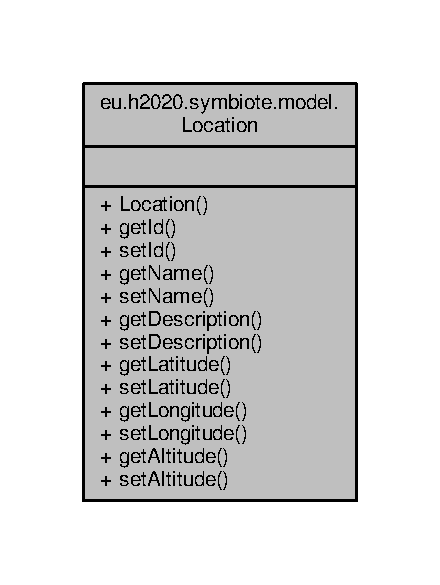
\includegraphics[width=211pt]{classeu_1_1h2020_1_1symbiote_1_1model_1_1Location__coll__graph}
\end{center}
\end{figure}
\subsection*{Public Member Functions}
\begin{DoxyCompactItemize}
\item 
String \hyperlink{classeu_1_1h2020_1_1symbiote_1_1model_1_1Location_a98a3b93d177deb7b9630c5e37547d80d}{get\+Id} ()
\item 
void \hyperlink{classeu_1_1h2020_1_1symbiote_1_1model_1_1Location_a308f71eeeed57f22b5996da217028d29}{set\+Id} (String id)
\item 
String \hyperlink{classeu_1_1h2020_1_1symbiote_1_1model_1_1Location_a78e563a2622952f37da6f571932afa23}{get\+Name} ()
\item 
void \hyperlink{classeu_1_1h2020_1_1symbiote_1_1model_1_1Location_a67ddf61270deeb669ebcdce9b9ead998}{set\+Name} (String name)
\item 
String \hyperlink{classeu_1_1h2020_1_1symbiote_1_1model_1_1Location_accf0bb0ab10306a962e09fc32c8d821c}{get\+Description} ()
\item 
void \hyperlink{classeu_1_1h2020_1_1symbiote_1_1model_1_1Location_a45d3f8f4397791af93669578501a43bf}{set\+Description} (String description)
\item 
double \hyperlink{classeu_1_1h2020_1_1symbiote_1_1model_1_1Location_a40812abe56323ccb3e65d1309d2d55e4}{get\+Latitude} ()
\item 
void \hyperlink{classeu_1_1h2020_1_1symbiote_1_1model_1_1Location_a26b8aab258d4422bd5fc64d7a512b685}{set\+Latitude} (double latitude)
\item 
double \hyperlink{classeu_1_1h2020_1_1symbiote_1_1model_1_1Location_afe9ac4993b9dbcc9350e2667e279d39b}{get\+Longitude} ()
\item 
void \hyperlink{classeu_1_1h2020_1_1symbiote_1_1model_1_1Location_a6bc9a04947915ea52001bccbcba0849e}{set\+Longitude} (double longitude)
\item 
double \hyperlink{classeu_1_1h2020_1_1symbiote_1_1model_1_1Location_a333c37abcd3c9ea766ca5ec6dddd5e3a}{get\+Altitude} ()
\item 
void \hyperlink{classeu_1_1h2020_1_1symbiote_1_1model_1_1Location_ac2fc6d59229ad7253416f2fdf650675d}{set\+Altitude} (double altitude)
\end{DoxyCompactItemize}


\subsection{Detailed Description}
Registry \hyperlink{classeu_1_1h2020_1_1symbiote_1_1model_1_1Location}{Location} object used with Resources.

Created by mateuszl 

\subsection{Member Function Documentation}
\index{eu\+::h2020\+::symbiote\+::model\+::\+Location@{eu\+::h2020\+::symbiote\+::model\+::\+Location}!get\+Altitude@{get\+Altitude}}
\index{get\+Altitude@{get\+Altitude}!eu\+::h2020\+::symbiote\+::model\+::\+Location@{eu\+::h2020\+::symbiote\+::model\+::\+Location}}
\subsubsection[{\texorpdfstring{get\+Altitude()}{getAltitude()}}]{\setlength{\rightskip}{0pt plus 5cm}double eu.\+h2020.\+symbiote.\+model.\+Location.\+get\+Altitude (
\begin{DoxyParamCaption}
{}
\end{DoxyParamCaption}
)}\hypertarget{classeu_1_1h2020_1_1symbiote_1_1model_1_1Location_a333c37abcd3c9ea766ca5ec6dddd5e3a}{}\label{classeu_1_1h2020_1_1symbiote_1_1model_1_1Location_a333c37abcd3c9ea766ca5ec6dddd5e3a}
\begin{DoxyReturn}{Returns}

\end{DoxyReturn}
\index{eu\+::h2020\+::symbiote\+::model\+::\+Location@{eu\+::h2020\+::symbiote\+::model\+::\+Location}!get\+Description@{get\+Description}}
\index{get\+Description@{get\+Description}!eu\+::h2020\+::symbiote\+::model\+::\+Location@{eu\+::h2020\+::symbiote\+::model\+::\+Location}}
\subsubsection[{\texorpdfstring{get\+Description()}{getDescription()}}]{\setlength{\rightskip}{0pt plus 5cm}String eu.\+h2020.\+symbiote.\+model.\+Location.\+get\+Description (
\begin{DoxyParamCaption}
{}
\end{DoxyParamCaption}
)}\hypertarget{classeu_1_1h2020_1_1symbiote_1_1model_1_1Location_accf0bb0ab10306a962e09fc32c8d821c}{}\label{classeu_1_1h2020_1_1symbiote_1_1model_1_1Location_accf0bb0ab10306a962e09fc32c8d821c}
\begin{DoxyReturn}{Returns}

\end{DoxyReturn}
\index{eu\+::h2020\+::symbiote\+::model\+::\+Location@{eu\+::h2020\+::symbiote\+::model\+::\+Location}!get\+Id@{get\+Id}}
\index{get\+Id@{get\+Id}!eu\+::h2020\+::symbiote\+::model\+::\+Location@{eu\+::h2020\+::symbiote\+::model\+::\+Location}}
\subsubsection[{\texorpdfstring{get\+Id()}{getId()}}]{\setlength{\rightskip}{0pt plus 5cm}String eu.\+h2020.\+symbiote.\+model.\+Location.\+get\+Id (
\begin{DoxyParamCaption}
{}
\end{DoxyParamCaption}
)}\hypertarget{classeu_1_1h2020_1_1symbiote_1_1model_1_1Location_a98a3b93d177deb7b9630c5e37547d80d}{}\label{classeu_1_1h2020_1_1symbiote_1_1model_1_1Location_a98a3b93d177deb7b9630c5e37547d80d}
\begin{DoxyReturn}{Returns}

\end{DoxyReturn}
\index{eu\+::h2020\+::symbiote\+::model\+::\+Location@{eu\+::h2020\+::symbiote\+::model\+::\+Location}!get\+Latitude@{get\+Latitude}}
\index{get\+Latitude@{get\+Latitude}!eu\+::h2020\+::symbiote\+::model\+::\+Location@{eu\+::h2020\+::symbiote\+::model\+::\+Location}}
\subsubsection[{\texorpdfstring{get\+Latitude()}{getLatitude()}}]{\setlength{\rightskip}{0pt plus 5cm}double eu.\+h2020.\+symbiote.\+model.\+Location.\+get\+Latitude (
\begin{DoxyParamCaption}
{}
\end{DoxyParamCaption}
)}\hypertarget{classeu_1_1h2020_1_1symbiote_1_1model_1_1Location_a40812abe56323ccb3e65d1309d2d55e4}{}\label{classeu_1_1h2020_1_1symbiote_1_1model_1_1Location_a40812abe56323ccb3e65d1309d2d55e4}
\begin{DoxyReturn}{Returns}

\end{DoxyReturn}
\index{eu\+::h2020\+::symbiote\+::model\+::\+Location@{eu\+::h2020\+::symbiote\+::model\+::\+Location}!get\+Longitude@{get\+Longitude}}
\index{get\+Longitude@{get\+Longitude}!eu\+::h2020\+::symbiote\+::model\+::\+Location@{eu\+::h2020\+::symbiote\+::model\+::\+Location}}
\subsubsection[{\texorpdfstring{get\+Longitude()}{getLongitude()}}]{\setlength{\rightskip}{0pt plus 5cm}double eu.\+h2020.\+symbiote.\+model.\+Location.\+get\+Longitude (
\begin{DoxyParamCaption}
{}
\end{DoxyParamCaption}
)}\hypertarget{classeu_1_1h2020_1_1symbiote_1_1model_1_1Location_afe9ac4993b9dbcc9350e2667e279d39b}{}\label{classeu_1_1h2020_1_1symbiote_1_1model_1_1Location_afe9ac4993b9dbcc9350e2667e279d39b}
\begin{DoxyReturn}{Returns}

\end{DoxyReturn}
\index{eu\+::h2020\+::symbiote\+::model\+::\+Location@{eu\+::h2020\+::symbiote\+::model\+::\+Location}!get\+Name@{get\+Name}}
\index{get\+Name@{get\+Name}!eu\+::h2020\+::symbiote\+::model\+::\+Location@{eu\+::h2020\+::symbiote\+::model\+::\+Location}}
\subsubsection[{\texorpdfstring{get\+Name()}{getName()}}]{\setlength{\rightskip}{0pt plus 5cm}String eu.\+h2020.\+symbiote.\+model.\+Location.\+get\+Name (
\begin{DoxyParamCaption}
{}
\end{DoxyParamCaption}
)}\hypertarget{classeu_1_1h2020_1_1symbiote_1_1model_1_1Location_a78e563a2622952f37da6f571932afa23}{}\label{classeu_1_1h2020_1_1symbiote_1_1model_1_1Location_a78e563a2622952f37da6f571932afa23}
\begin{DoxyReturn}{Returns}

\end{DoxyReturn}
\index{eu\+::h2020\+::symbiote\+::model\+::\+Location@{eu\+::h2020\+::symbiote\+::model\+::\+Location}!set\+Altitude@{set\+Altitude}}
\index{set\+Altitude@{set\+Altitude}!eu\+::h2020\+::symbiote\+::model\+::\+Location@{eu\+::h2020\+::symbiote\+::model\+::\+Location}}
\subsubsection[{\texorpdfstring{set\+Altitude(double altitude)}{setAltitude(double altitude)}}]{\setlength{\rightskip}{0pt plus 5cm}void eu.\+h2020.\+symbiote.\+model.\+Location.\+set\+Altitude (
\begin{DoxyParamCaption}
\item[{double}]{altitude}
\end{DoxyParamCaption}
)}\hypertarget{classeu_1_1h2020_1_1symbiote_1_1model_1_1Location_ac2fc6d59229ad7253416f2fdf650675d}{}\label{classeu_1_1h2020_1_1symbiote_1_1model_1_1Location_ac2fc6d59229ad7253416f2fdf650675d}

\begin{DoxyParams}{Parameters}
{\em altitude} & \\
\hline
\end{DoxyParams}
\index{eu\+::h2020\+::symbiote\+::model\+::\+Location@{eu\+::h2020\+::symbiote\+::model\+::\+Location}!set\+Description@{set\+Description}}
\index{set\+Description@{set\+Description}!eu\+::h2020\+::symbiote\+::model\+::\+Location@{eu\+::h2020\+::symbiote\+::model\+::\+Location}}
\subsubsection[{\texorpdfstring{set\+Description(\+String description)}{setDescription(String description)}}]{\setlength{\rightskip}{0pt plus 5cm}void eu.\+h2020.\+symbiote.\+model.\+Location.\+set\+Description (
\begin{DoxyParamCaption}
\item[{String}]{description}
\end{DoxyParamCaption}
)}\hypertarget{classeu_1_1h2020_1_1symbiote_1_1model_1_1Location_a45d3f8f4397791af93669578501a43bf}{}\label{classeu_1_1h2020_1_1symbiote_1_1model_1_1Location_a45d3f8f4397791af93669578501a43bf}

\begin{DoxyParams}{Parameters}
{\em description} & \\
\hline
\end{DoxyParams}
\index{eu\+::h2020\+::symbiote\+::model\+::\+Location@{eu\+::h2020\+::symbiote\+::model\+::\+Location}!set\+Id@{set\+Id}}
\index{set\+Id@{set\+Id}!eu\+::h2020\+::symbiote\+::model\+::\+Location@{eu\+::h2020\+::symbiote\+::model\+::\+Location}}
\subsubsection[{\texorpdfstring{set\+Id(\+String id)}{setId(String id)}}]{\setlength{\rightskip}{0pt plus 5cm}void eu.\+h2020.\+symbiote.\+model.\+Location.\+set\+Id (
\begin{DoxyParamCaption}
\item[{String}]{id}
\end{DoxyParamCaption}
)}\hypertarget{classeu_1_1h2020_1_1symbiote_1_1model_1_1Location_a308f71eeeed57f22b5996da217028d29}{}\label{classeu_1_1h2020_1_1symbiote_1_1model_1_1Location_a308f71eeeed57f22b5996da217028d29}

\begin{DoxyParams}{Parameters}
{\em id} & \\
\hline
\end{DoxyParams}
\index{eu\+::h2020\+::symbiote\+::model\+::\+Location@{eu\+::h2020\+::symbiote\+::model\+::\+Location}!set\+Latitude@{set\+Latitude}}
\index{set\+Latitude@{set\+Latitude}!eu\+::h2020\+::symbiote\+::model\+::\+Location@{eu\+::h2020\+::symbiote\+::model\+::\+Location}}
\subsubsection[{\texorpdfstring{set\+Latitude(double latitude)}{setLatitude(double latitude)}}]{\setlength{\rightskip}{0pt plus 5cm}void eu.\+h2020.\+symbiote.\+model.\+Location.\+set\+Latitude (
\begin{DoxyParamCaption}
\item[{double}]{latitude}
\end{DoxyParamCaption}
)}\hypertarget{classeu_1_1h2020_1_1symbiote_1_1model_1_1Location_a26b8aab258d4422bd5fc64d7a512b685}{}\label{classeu_1_1h2020_1_1symbiote_1_1model_1_1Location_a26b8aab258d4422bd5fc64d7a512b685}

\begin{DoxyParams}{Parameters}
{\em latitude} & \\
\hline
\end{DoxyParams}
\index{eu\+::h2020\+::symbiote\+::model\+::\+Location@{eu\+::h2020\+::symbiote\+::model\+::\+Location}!set\+Longitude@{set\+Longitude}}
\index{set\+Longitude@{set\+Longitude}!eu\+::h2020\+::symbiote\+::model\+::\+Location@{eu\+::h2020\+::symbiote\+::model\+::\+Location}}
\subsubsection[{\texorpdfstring{set\+Longitude(double longitude)}{setLongitude(double longitude)}}]{\setlength{\rightskip}{0pt plus 5cm}void eu.\+h2020.\+symbiote.\+model.\+Location.\+set\+Longitude (
\begin{DoxyParamCaption}
\item[{double}]{longitude}
\end{DoxyParamCaption}
)}\hypertarget{classeu_1_1h2020_1_1symbiote_1_1model_1_1Location_a6bc9a04947915ea52001bccbcba0849e}{}\label{classeu_1_1h2020_1_1symbiote_1_1model_1_1Location_a6bc9a04947915ea52001bccbcba0849e}

\begin{DoxyParams}{Parameters}
{\em longitude} & \\
\hline
\end{DoxyParams}
\index{eu\+::h2020\+::symbiote\+::model\+::\+Location@{eu\+::h2020\+::symbiote\+::model\+::\+Location}!set\+Name@{set\+Name}}
\index{set\+Name@{set\+Name}!eu\+::h2020\+::symbiote\+::model\+::\+Location@{eu\+::h2020\+::symbiote\+::model\+::\+Location}}
\subsubsection[{\texorpdfstring{set\+Name(\+String name)}{setName(String name)}}]{\setlength{\rightskip}{0pt plus 5cm}void eu.\+h2020.\+symbiote.\+model.\+Location.\+set\+Name (
\begin{DoxyParamCaption}
\item[{String}]{name}
\end{DoxyParamCaption}
)}\hypertarget{classeu_1_1h2020_1_1symbiote_1_1model_1_1Location_a67ddf61270deeb669ebcdce9b9ead998}{}\label{classeu_1_1h2020_1_1symbiote_1_1model_1_1Location_a67ddf61270deeb669ebcdce9b9ead998}

\begin{DoxyParams}{Parameters}
{\em name} & \\
\hline
\end{DoxyParams}


The documentation for this class was generated from the following file\+:\begin{DoxyCompactItemize}
\item 
src/main/java/eu/h2020/symbiote/model/Location.\+java\end{DoxyCompactItemize}

\hypertarget{interfaceeu_1_1h2020_1_1symbiote_1_1repository_1_1LocationRepository}{}\section{eu.\+h2020.\+symbiote.\+repository.\+Location\+Repository Interface Reference}
\label{interfaceeu_1_1h2020_1_1symbiote_1_1repository_1_1LocationRepository}\index{eu.\+h2020.\+symbiote.\+repository.\+Location\+Repository@{eu.\+h2020.\+symbiote.\+repository.\+Location\+Repository}}


Inheritance diagram for eu.\+h2020.\+symbiote.\+repository.\+Location\+Repository\+:
% FIG 0


Collaboration diagram for eu.\+h2020.\+symbiote.\+repository.\+Location\+Repository\+:
% FIG 1


\subsection{Detailed Description}
Registry Mongo\+DB Persistence layer for Location objects

Created by mateuszl 

The documentation for this interface was generated from the following file\+:\begin{DoxyCompactItemize}
\item 
src/main/java/eu/h2020/symbiote/repository/Location\+Repository.\+java\end{DoxyCompactItemize}

\hypertarget{classeu_1_1h2020_1_1symbiote_1_1model_1_1Platform}{}\section{eu.\+h2020.\+symbiote.\+model.\+Platform Class Reference}
\label{classeu_1_1h2020_1_1symbiote_1_1model_1_1Platform}\index{eu.\+h2020.\+symbiote.\+model.\+Platform@{eu.\+h2020.\+symbiote.\+model.\+Platform}}


Collaboration diagram for eu.\+h2020.\+symbiote.\+model.\+Platform\+:
% FIG 0
\subsection*{Public Member Functions}
\begin{DoxyCompactItemize}
\item 
String \hyperlink{classeu_1_1h2020_1_1symbiote_1_1model_1_1Platform_a2a09b94af05846adcf58f6405f0b1fdc}{get\+Platform\+Id} ()
\item 
void \hyperlink{classeu_1_1h2020_1_1symbiote_1_1model_1_1Platform_a3d9e886790d506f713e997f3c587e8ac}{set\+Platform\+Id} (String platform\+Id)
\item 
String \hyperlink{classeu_1_1h2020_1_1symbiote_1_1model_1_1Platform_a9d39e85c470888c7043448f2eb059325}{get\+Name} ()
\item 
void \hyperlink{classeu_1_1h2020_1_1symbiote_1_1model_1_1Platform_af4d5506c08659b3d71dcc8bf69c743ce}{set\+Name} (String name)
\item 
String \hyperlink{classeu_1_1h2020_1_1symbiote_1_1model_1_1Platform_ad4a8d6cbb5ed57e241f783c512f052d9}{get\+Description} ()
\item 
void \hyperlink{classeu_1_1h2020_1_1symbiote_1_1model_1_1Platform_a9ec81f09b9fcd25ae264618591992cb2}{set\+Description} (String description)
\item 
String \hyperlink{classeu_1_1h2020_1_1symbiote_1_1model_1_1Platform_a4ca440b89e37c323dcb812ef07cfb66a}{get\+Url} ()
\item 
void \hyperlink{classeu_1_1h2020_1_1symbiote_1_1model_1_1Platform_ac4d39a74475da2c2318cfd5e3667a5a1}{set\+Url} (String url)
\item 
String \hyperlink{classeu_1_1h2020_1_1symbiote_1_1model_1_1Platform_a799a5bb8e0665457c4b8bfd2b34c9b3c}{get\+Information\+Model\+Id} ()
\item 
void \hyperlink{classeu_1_1h2020_1_1symbiote_1_1model_1_1Platform_ae3e1cb93bcb289d575f215990d7e9499}{set\+Information\+Model\+Id} (String information\+Model\+Id)
\item 
int {\bfseries hash\+Code} ()\hypertarget{classeu_1_1h2020_1_1symbiote_1_1model_1_1Platform_a3b85d6919db55e5a8584a909a4599953}{}\label{classeu_1_1h2020_1_1symbiote_1_1model_1_1Platform_a3b85d6919db55e5a8584a909a4599953}

\item 
boolean {\bfseries equals} (Object obj)\hypertarget{classeu_1_1h2020_1_1symbiote_1_1model_1_1Platform_ab00da56375115817b0594f8865667d30}{}\label{classeu_1_1h2020_1_1symbiote_1_1model_1_1Platform_ab00da56375115817b0594f8865667d30}

\end{DoxyCompactItemize}


\subsection{Detailed Description}
Registry \hyperlink{classeu_1_1h2020_1_1symbiote_1_1model_1_1Platform}{Platform} object

Created by mateuszl 

\subsection{Member Function Documentation}
\index{eu\+::h2020\+::symbiote\+::model\+::\+Platform@{eu\+::h2020\+::symbiote\+::model\+::\+Platform}!get\+Description@{get\+Description}}
\index{get\+Description@{get\+Description}!eu\+::h2020\+::symbiote\+::model\+::\+Platform@{eu\+::h2020\+::symbiote\+::model\+::\+Platform}}
\subsubsection[{\texorpdfstring{get\+Description()}{getDescription()}}]{\setlength{\rightskip}{0pt plus 5cm}String eu.\+h2020.\+symbiote.\+model.\+Platform.\+get\+Description (
\begin{DoxyParamCaption}
{}
\end{DoxyParamCaption}
)}\hypertarget{classeu_1_1h2020_1_1symbiote_1_1model_1_1Platform_ad4a8d6cbb5ed57e241f783c512f052d9}{}\label{classeu_1_1h2020_1_1symbiote_1_1model_1_1Platform_ad4a8d6cbb5ed57e241f783c512f052d9}
\begin{DoxyReturn}{Returns}

\end{DoxyReturn}
\index{eu\+::h2020\+::symbiote\+::model\+::\+Platform@{eu\+::h2020\+::symbiote\+::model\+::\+Platform}!get\+Information\+Model\+Id@{get\+Information\+Model\+Id}}
\index{get\+Information\+Model\+Id@{get\+Information\+Model\+Id}!eu\+::h2020\+::symbiote\+::model\+::\+Platform@{eu\+::h2020\+::symbiote\+::model\+::\+Platform}}
\subsubsection[{\texorpdfstring{get\+Information\+Model\+Id()}{getInformationModelId()}}]{\setlength{\rightskip}{0pt plus 5cm}String eu.\+h2020.\+symbiote.\+model.\+Platform.\+get\+Information\+Model\+Id (
\begin{DoxyParamCaption}
{}
\end{DoxyParamCaption}
)}\hypertarget{classeu_1_1h2020_1_1symbiote_1_1model_1_1Platform_a799a5bb8e0665457c4b8bfd2b34c9b3c}{}\label{classeu_1_1h2020_1_1symbiote_1_1model_1_1Platform_a799a5bb8e0665457c4b8bfd2b34c9b3c}
\begin{DoxyReturn}{Returns}

\end{DoxyReturn}
\index{eu\+::h2020\+::symbiote\+::model\+::\+Platform@{eu\+::h2020\+::symbiote\+::model\+::\+Platform}!get\+Name@{get\+Name}}
\index{get\+Name@{get\+Name}!eu\+::h2020\+::symbiote\+::model\+::\+Platform@{eu\+::h2020\+::symbiote\+::model\+::\+Platform}}
\subsubsection[{\texorpdfstring{get\+Name()}{getName()}}]{\setlength{\rightskip}{0pt plus 5cm}String eu.\+h2020.\+symbiote.\+model.\+Platform.\+get\+Name (
\begin{DoxyParamCaption}
{}
\end{DoxyParamCaption}
)}\hypertarget{classeu_1_1h2020_1_1symbiote_1_1model_1_1Platform_a9d39e85c470888c7043448f2eb059325}{}\label{classeu_1_1h2020_1_1symbiote_1_1model_1_1Platform_a9d39e85c470888c7043448f2eb059325}
\begin{DoxyReturn}{Returns}

\end{DoxyReturn}
\index{eu\+::h2020\+::symbiote\+::model\+::\+Platform@{eu\+::h2020\+::symbiote\+::model\+::\+Platform}!get\+Platform\+Id@{get\+Platform\+Id}}
\index{get\+Platform\+Id@{get\+Platform\+Id}!eu\+::h2020\+::symbiote\+::model\+::\+Platform@{eu\+::h2020\+::symbiote\+::model\+::\+Platform}}
\subsubsection[{\texorpdfstring{get\+Platform\+Id()}{getPlatformId()}}]{\setlength{\rightskip}{0pt plus 5cm}String eu.\+h2020.\+symbiote.\+model.\+Platform.\+get\+Platform\+Id (
\begin{DoxyParamCaption}
{}
\end{DoxyParamCaption}
)}\hypertarget{classeu_1_1h2020_1_1symbiote_1_1model_1_1Platform_a2a09b94af05846adcf58f6405f0b1fdc}{}\label{classeu_1_1h2020_1_1symbiote_1_1model_1_1Platform_a2a09b94af05846adcf58f6405f0b1fdc}
\begin{DoxyReturn}{Returns}

\end{DoxyReturn}
\index{eu\+::h2020\+::symbiote\+::model\+::\+Platform@{eu\+::h2020\+::symbiote\+::model\+::\+Platform}!get\+Url@{get\+Url}}
\index{get\+Url@{get\+Url}!eu\+::h2020\+::symbiote\+::model\+::\+Platform@{eu\+::h2020\+::symbiote\+::model\+::\+Platform}}
\subsubsection[{\texorpdfstring{get\+Url()}{getUrl()}}]{\setlength{\rightskip}{0pt plus 5cm}String eu.\+h2020.\+symbiote.\+model.\+Platform.\+get\+Url (
\begin{DoxyParamCaption}
{}
\end{DoxyParamCaption}
)}\hypertarget{classeu_1_1h2020_1_1symbiote_1_1model_1_1Platform_a4ca440b89e37c323dcb812ef07cfb66a}{}\label{classeu_1_1h2020_1_1symbiote_1_1model_1_1Platform_a4ca440b89e37c323dcb812ef07cfb66a}
\begin{DoxyReturn}{Returns}

\end{DoxyReturn}
\index{eu\+::h2020\+::symbiote\+::model\+::\+Platform@{eu\+::h2020\+::symbiote\+::model\+::\+Platform}!set\+Description@{set\+Description}}
\index{set\+Description@{set\+Description}!eu\+::h2020\+::symbiote\+::model\+::\+Platform@{eu\+::h2020\+::symbiote\+::model\+::\+Platform}}
\subsubsection[{\texorpdfstring{set\+Description(\+String description)}{setDescription(String description)}}]{\setlength{\rightskip}{0pt plus 5cm}void eu.\+h2020.\+symbiote.\+model.\+Platform.\+set\+Description (
\begin{DoxyParamCaption}
\item[{String}]{description}
\end{DoxyParamCaption}
)}\hypertarget{classeu_1_1h2020_1_1symbiote_1_1model_1_1Platform_a9ec81f09b9fcd25ae264618591992cb2}{}\label{classeu_1_1h2020_1_1symbiote_1_1model_1_1Platform_a9ec81f09b9fcd25ae264618591992cb2}

\begin{DoxyParams}{Parameters}
{\em description} & \\
\hline
\end{DoxyParams}
\index{eu\+::h2020\+::symbiote\+::model\+::\+Platform@{eu\+::h2020\+::symbiote\+::model\+::\+Platform}!set\+Information\+Model\+Id@{set\+Information\+Model\+Id}}
\index{set\+Information\+Model\+Id@{set\+Information\+Model\+Id}!eu\+::h2020\+::symbiote\+::model\+::\+Platform@{eu\+::h2020\+::symbiote\+::model\+::\+Platform}}
\subsubsection[{\texorpdfstring{set\+Information\+Model\+Id(\+String information\+Model\+Id)}{setInformationModelId(String informationModelId)}}]{\setlength{\rightskip}{0pt plus 5cm}void eu.\+h2020.\+symbiote.\+model.\+Platform.\+set\+Information\+Model\+Id (
\begin{DoxyParamCaption}
\item[{String}]{information\+Model\+Id}
\end{DoxyParamCaption}
)}\hypertarget{classeu_1_1h2020_1_1symbiote_1_1model_1_1Platform_ae3e1cb93bcb289d575f215990d7e9499}{}\label{classeu_1_1h2020_1_1symbiote_1_1model_1_1Platform_ae3e1cb93bcb289d575f215990d7e9499}

\begin{DoxyParams}{Parameters}
{\em information\+Model\+Id} & \\
\hline
\end{DoxyParams}
\index{eu\+::h2020\+::symbiote\+::model\+::\+Platform@{eu\+::h2020\+::symbiote\+::model\+::\+Platform}!set\+Name@{set\+Name}}
\index{set\+Name@{set\+Name}!eu\+::h2020\+::symbiote\+::model\+::\+Platform@{eu\+::h2020\+::symbiote\+::model\+::\+Platform}}
\subsubsection[{\texorpdfstring{set\+Name(\+String name)}{setName(String name)}}]{\setlength{\rightskip}{0pt plus 5cm}void eu.\+h2020.\+symbiote.\+model.\+Platform.\+set\+Name (
\begin{DoxyParamCaption}
\item[{String}]{name}
\end{DoxyParamCaption}
)}\hypertarget{classeu_1_1h2020_1_1symbiote_1_1model_1_1Platform_af4d5506c08659b3d71dcc8bf69c743ce}{}\label{classeu_1_1h2020_1_1symbiote_1_1model_1_1Platform_af4d5506c08659b3d71dcc8bf69c743ce}

\begin{DoxyParams}{Parameters}
{\em name} & \\
\hline
\end{DoxyParams}
\index{eu\+::h2020\+::symbiote\+::model\+::\+Platform@{eu\+::h2020\+::symbiote\+::model\+::\+Platform}!set\+Platform\+Id@{set\+Platform\+Id}}
\index{set\+Platform\+Id@{set\+Platform\+Id}!eu\+::h2020\+::symbiote\+::model\+::\+Platform@{eu\+::h2020\+::symbiote\+::model\+::\+Platform}}
\subsubsection[{\texorpdfstring{set\+Platform\+Id(\+String platform\+Id)}{setPlatformId(String platformId)}}]{\setlength{\rightskip}{0pt plus 5cm}void eu.\+h2020.\+symbiote.\+model.\+Platform.\+set\+Platform\+Id (
\begin{DoxyParamCaption}
\item[{String}]{platform\+Id}
\end{DoxyParamCaption}
)}\hypertarget{classeu_1_1h2020_1_1symbiote_1_1model_1_1Platform_a3d9e886790d506f713e997f3c587e8ac}{}\label{classeu_1_1h2020_1_1symbiote_1_1model_1_1Platform_a3d9e886790d506f713e997f3c587e8ac}

\begin{DoxyParams}{Parameters}
{\em platform\+Id} & \\
\hline
\end{DoxyParams}
\index{eu\+::h2020\+::symbiote\+::model\+::\+Platform@{eu\+::h2020\+::symbiote\+::model\+::\+Platform}!set\+Url@{set\+Url}}
\index{set\+Url@{set\+Url}!eu\+::h2020\+::symbiote\+::model\+::\+Platform@{eu\+::h2020\+::symbiote\+::model\+::\+Platform}}
\subsubsection[{\texorpdfstring{set\+Url(\+String url)}{setUrl(String url)}}]{\setlength{\rightskip}{0pt plus 5cm}void eu.\+h2020.\+symbiote.\+model.\+Platform.\+set\+Url (
\begin{DoxyParamCaption}
\item[{String}]{url}
\end{DoxyParamCaption}
)}\hypertarget{classeu_1_1h2020_1_1symbiote_1_1model_1_1Platform_ac4d39a74475da2c2318cfd5e3667a5a1}{}\label{classeu_1_1h2020_1_1symbiote_1_1model_1_1Platform_ac4d39a74475da2c2318cfd5e3667a5a1}

\begin{DoxyParams}{Parameters}
{\em url} & \\
\hline
\end{DoxyParams}


The documentation for this class was generated from the following file\+:\begin{DoxyCompactItemize}
\item 
src/main/java/eu/h2020/symbiote/model/Platform.\+java\end{DoxyCompactItemize}

\hypertarget{classeu_1_1h2020_1_1symbiote_1_1messaging_1_1PlatformCreationRequestConsumer}{}\section{eu.\+h2020.\+symbiote.\+messaging.\+Platform\+Creation\+Request\+Consumer Class Reference}
\label{classeu_1_1h2020_1_1symbiote_1_1messaging_1_1PlatformCreationRequestConsumer}\index{eu.\+h2020.\+symbiote.\+messaging.\+Platform\+Creation\+Request\+Consumer@{eu.\+h2020.\+symbiote.\+messaging.\+Platform\+Creation\+Request\+Consumer}}


Inheritance diagram for eu.\+h2020.\+symbiote.\+messaging.\+Platform\+Creation\+Request\+Consumer\+:
\nopagebreak
\begin{figure}[H]
\begin{center}
\leavevmode
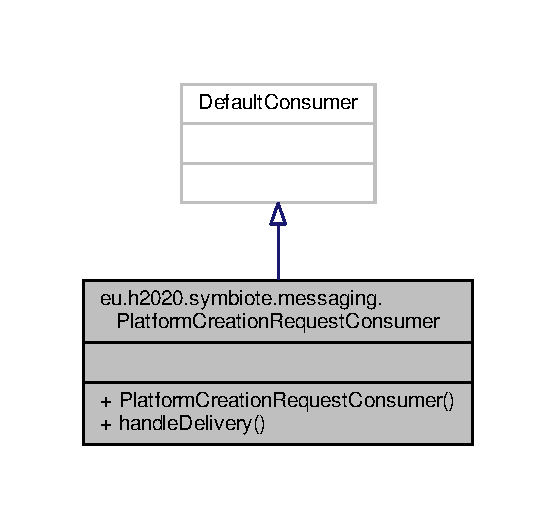
\includegraphics[width=267pt]{classeu_1_1h2020_1_1symbiote_1_1messaging_1_1PlatformCreationRequestConsumer__inherit__graph}
\end{center}
\end{figure}


Collaboration diagram for eu.\+h2020.\+symbiote.\+messaging.\+Platform\+Creation\+Request\+Consumer\+:
\nopagebreak
\begin{figure}[H]
\begin{center}
\leavevmode
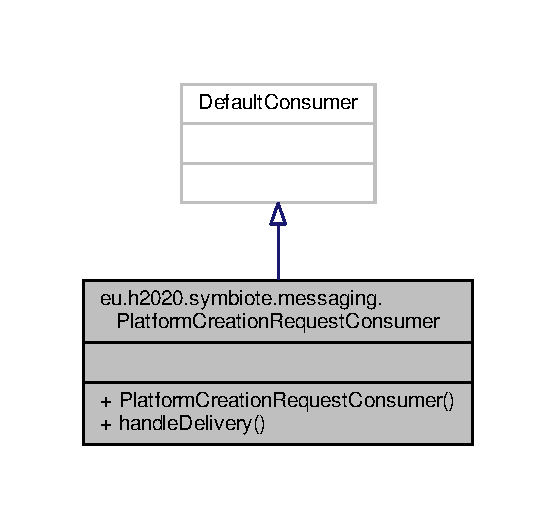
\includegraphics[width=267pt]{classeu_1_1h2020_1_1symbiote_1_1messaging_1_1PlatformCreationRequestConsumer__coll__graph}
\end{center}
\end{figure}
\subsection*{Public Member Functions}
\begin{DoxyCompactItemize}
\item 
\hyperlink{classeu_1_1h2020_1_1symbiote_1_1messaging_1_1PlatformCreationRequestConsumer_ac7f4497c390c067a2e42196b0e050bf9}{Platform\+Creation\+Request\+Consumer} (Channel channel, \hyperlink{classeu_1_1h2020_1_1symbiote_1_1repository_1_1RepositoryManager}{Repository\+Manager} repository\+Manager, \hyperlink{classeu_1_1h2020_1_1symbiote_1_1messaging_1_1RabbitManager}{Rabbit\+Manager} rabbit\+Manager)
\item 
void \hyperlink{classeu_1_1h2020_1_1symbiote_1_1messaging_1_1PlatformCreationRequestConsumer_a5effadb30758abb5f438be74a6c7f054}{handle\+Delivery} (String consumer\+Tag, Envelope envelope, A\+M\+Q\+P.\+Basic\+Properties properties, byte\mbox{[}$\,$\mbox{]} body)  throws I\+O\+Exception 
\end{DoxyCompactItemize}


\subsection{Detailed Description}
Rabbit\+MQ Consumer implementation used for Platform Creation actions

Created by mateuszl 

\subsection{Constructor \& Destructor Documentation}
\index{eu\+::h2020\+::symbiote\+::messaging\+::\+Platform\+Creation\+Request\+Consumer@{eu\+::h2020\+::symbiote\+::messaging\+::\+Platform\+Creation\+Request\+Consumer}!Platform\+Creation\+Request\+Consumer@{Platform\+Creation\+Request\+Consumer}}
\index{Platform\+Creation\+Request\+Consumer@{Platform\+Creation\+Request\+Consumer}!eu\+::h2020\+::symbiote\+::messaging\+::\+Platform\+Creation\+Request\+Consumer@{eu\+::h2020\+::symbiote\+::messaging\+::\+Platform\+Creation\+Request\+Consumer}}
\subsubsection[{\texorpdfstring{Platform\+Creation\+Request\+Consumer(\+Channel channel, Repository\+Manager repository\+Manager, Rabbit\+Manager rabbit\+Manager)}{PlatformCreationRequestConsumer(Channel channel, RepositoryManager repositoryManager, RabbitManager rabbitManager)}}]{\setlength{\rightskip}{0pt plus 5cm}eu.\+h2020.\+symbiote.\+messaging.\+Platform\+Creation\+Request\+Consumer.\+Platform\+Creation\+Request\+Consumer (
\begin{DoxyParamCaption}
\item[{Channel}]{channel, }
\item[{{\bf Repository\+Manager}}]{repository\+Manager, }
\item[{{\bf Rabbit\+Manager}}]{rabbit\+Manager}
\end{DoxyParamCaption}
)}\hypertarget{classeu_1_1h2020_1_1symbiote_1_1messaging_1_1PlatformCreationRequestConsumer_ac7f4497c390c067a2e42196b0e050bf9}{}\label{classeu_1_1h2020_1_1symbiote_1_1messaging_1_1PlatformCreationRequestConsumer_ac7f4497c390c067a2e42196b0e050bf9}
Constructs a new instance and records its association to the passed-\/in channel. Managers beans passed as parameters because of lack of possibility to inject it to consumer.


\begin{DoxyParams}{Parameters}
{\em channel} & the channel to which this consumer is attached \\
\hline
{\em rabbit\+Manager} & rabbit manager bean passed for access to messages manager \\
\hline
{\em repository\+Manager} & repository manager bean passed for persistence actions \\
\hline
\end{DoxyParams}


\subsection{Member Function Documentation}
\index{eu\+::h2020\+::symbiote\+::messaging\+::\+Platform\+Creation\+Request\+Consumer@{eu\+::h2020\+::symbiote\+::messaging\+::\+Platform\+Creation\+Request\+Consumer}!handle\+Delivery@{handle\+Delivery}}
\index{handle\+Delivery@{handle\+Delivery}!eu\+::h2020\+::symbiote\+::messaging\+::\+Platform\+Creation\+Request\+Consumer@{eu\+::h2020\+::symbiote\+::messaging\+::\+Platform\+Creation\+Request\+Consumer}}
\subsubsection[{\texorpdfstring{handle\+Delivery(\+String consumer\+Tag, Envelope envelope, A\+M\+Q\+P.\+Basic\+Properties properties, byte[] body)}{handleDelivery(String consumerTag, Envelope envelope, AMQP.BasicProperties properties, byte[] body)}}]{\setlength{\rightskip}{0pt plus 5cm}void eu.\+h2020.\+symbiote.\+messaging.\+Platform\+Creation\+Request\+Consumer.\+handle\+Delivery (
\begin{DoxyParamCaption}
\item[{String}]{consumer\+Tag, }
\item[{Envelope}]{envelope, }
\item[{A\+M\+Q\+P.\+Basic\+Properties}]{properties, }
\item[{byte\mbox{[}$\,$\mbox{]}}]{body}
\end{DoxyParamCaption}
) throws I\+O\+Exception}\hypertarget{classeu_1_1h2020_1_1symbiote_1_1messaging_1_1PlatformCreationRequestConsumer_a5effadb30758abb5f438be74a6c7f054}{}\label{classeu_1_1h2020_1_1symbiote_1_1messaging_1_1PlatformCreationRequestConsumer_a5effadb30758abb5f438be74a6c7f054}
Called when a {\ttfamily {\bfseries basic.\+deliver}} is received for this consumer.


\begin{DoxyParams}{Parameters}
{\em consumer\+Tag} & the {\itshape consumer tag} associated with the consumer \\
\hline
{\em envelope} & packaging data for the message \\
\hline
{\em properties} & content header data for the message \\
\hline
{\em body} & the message body (opaque, client-\/specific byte array) \\
\hline
\end{DoxyParams}

\begin{DoxyExceptions}{Exceptions}
{\em I\+O\+Exception} & if the consumer encounters an I/O error while processing the message \\
\hline
\end{DoxyExceptions}
\begin{DoxySeeAlso}{See also}
Envelope 
\end{DoxySeeAlso}


The documentation for this class was generated from the following file\+:\begin{DoxyCompactItemize}
\item 
src/main/java/eu/h2020/symbiote/messaging/Platform\+Creation\+Request\+Consumer.\+java\end{DoxyCompactItemize}

\hypertarget{classeu_1_1h2020_1_1symbiote_1_1messaging_1_1PlatformModificationRequestConsumer}{}\section{eu.\+h2020.\+symbiote.\+messaging.\+Platform\+Modification\+Request\+Consumer Class Reference}
\label{classeu_1_1h2020_1_1symbiote_1_1messaging_1_1PlatformModificationRequestConsumer}\index{eu.\+h2020.\+symbiote.\+messaging.\+Platform\+Modification\+Request\+Consumer@{eu.\+h2020.\+symbiote.\+messaging.\+Platform\+Modification\+Request\+Consumer}}


Inheritance diagram for eu.\+h2020.\+symbiote.\+messaging.\+Platform\+Modification\+Request\+Consumer\+:
% FIG 0


Collaboration diagram for eu.\+h2020.\+symbiote.\+messaging.\+Platform\+Modification\+Request\+Consumer\+:
% FIG 1
\subsection*{Public Member Functions}
\begin{DoxyCompactItemize}
\item 
\hyperlink{classeu_1_1h2020_1_1symbiote_1_1messaging_1_1PlatformModificationRequestConsumer_a68aef30b8dec1bfee5049027aadb0d28}{Platform\+Modification\+Request\+Consumer} (Channel channel, \hyperlink{classeu_1_1h2020_1_1symbiote_1_1repository_1_1RepositoryManager}{Repository\+Manager} repository\+Manager, \hyperlink{classeu_1_1h2020_1_1symbiote_1_1messaging_1_1RabbitManager}{Rabbit\+Manager} rabbit\+Manager)
\item 
void \hyperlink{classeu_1_1h2020_1_1symbiote_1_1messaging_1_1PlatformModificationRequestConsumer_abd849a1e55f280762f4571d4214004a3}{handle\+Delivery} (String consumer\+Tag, Envelope envelope, A\+M\+Q\+P.\+Basic\+Properties properties, byte\mbox{[}$\,$\mbox{]} body)  throws I\+O\+Exception 
\end{DoxyCompactItemize}


\subsection{Detailed Description}
Rabbit\+MQ Consumer implementation used for Platform Modification actions 

\subsection{Constructor \& Destructor Documentation}
\index{eu\+::h2020\+::symbiote\+::messaging\+::\+Platform\+Modification\+Request\+Consumer@{eu\+::h2020\+::symbiote\+::messaging\+::\+Platform\+Modification\+Request\+Consumer}!Platform\+Modification\+Request\+Consumer@{Platform\+Modification\+Request\+Consumer}}
\index{Platform\+Modification\+Request\+Consumer@{Platform\+Modification\+Request\+Consumer}!eu\+::h2020\+::symbiote\+::messaging\+::\+Platform\+Modification\+Request\+Consumer@{eu\+::h2020\+::symbiote\+::messaging\+::\+Platform\+Modification\+Request\+Consumer}}
\subsubsection[{\texorpdfstring{Platform\+Modification\+Request\+Consumer(\+Channel channel, Repository\+Manager repository\+Manager, Rabbit\+Manager rabbit\+Manager)}{PlatformModificationRequestConsumer(Channel channel, RepositoryManager repositoryManager, RabbitManager rabbitManager)}}]{\setlength{\rightskip}{0pt plus 5cm}eu.\+h2020.\+symbiote.\+messaging.\+Platform\+Modification\+Request\+Consumer.\+Platform\+Modification\+Request\+Consumer (
\begin{DoxyParamCaption}
\item[{Channel}]{channel, }
\item[{{\bf Repository\+Manager}}]{repository\+Manager, }
\item[{{\bf Rabbit\+Manager}}]{rabbit\+Manager}
\end{DoxyParamCaption}
)}\hypertarget{classeu_1_1h2020_1_1symbiote_1_1messaging_1_1PlatformModificationRequestConsumer_a68aef30b8dec1bfee5049027aadb0d28}{}\label{classeu_1_1h2020_1_1symbiote_1_1messaging_1_1PlatformModificationRequestConsumer_a68aef30b8dec1bfee5049027aadb0d28}
Constructs a new instance and records its association to the passed-\/in channel. Managers beans passed as parameters because of lack of possibility to inject it to consumer.


\begin{DoxyParams}{Parameters}
{\em channel} & the channel to which this consumer is attached \\
\hline
{\em rabbit\+Manager} & rabbit manager bean passed for access to messages manager \\
\hline
{\em repository\+Manager} & repository manager bean passed for persistence actions \\
\hline
\end{DoxyParams}


\subsection{Member Function Documentation}
\index{eu\+::h2020\+::symbiote\+::messaging\+::\+Platform\+Modification\+Request\+Consumer@{eu\+::h2020\+::symbiote\+::messaging\+::\+Platform\+Modification\+Request\+Consumer}!handle\+Delivery@{handle\+Delivery}}
\index{handle\+Delivery@{handle\+Delivery}!eu\+::h2020\+::symbiote\+::messaging\+::\+Platform\+Modification\+Request\+Consumer@{eu\+::h2020\+::symbiote\+::messaging\+::\+Platform\+Modification\+Request\+Consumer}}
\subsubsection[{\texorpdfstring{handle\+Delivery(\+String consumer\+Tag, Envelope envelope, A\+M\+Q\+P.\+Basic\+Properties properties, byte[] body)}{handleDelivery(String consumerTag, Envelope envelope, AMQP.BasicProperties properties, byte[] body)}}]{\setlength{\rightskip}{0pt plus 5cm}void eu.\+h2020.\+symbiote.\+messaging.\+Platform\+Modification\+Request\+Consumer.\+handle\+Delivery (
\begin{DoxyParamCaption}
\item[{String}]{consumer\+Tag, }
\item[{Envelope}]{envelope, }
\item[{A\+M\+Q\+P.\+Basic\+Properties}]{properties, }
\item[{byte\mbox{[}$\,$\mbox{]}}]{body}
\end{DoxyParamCaption}
) throws I\+O\+Exception}\hypertarget{classeu_1_1h2020_1_1symbiote_1_1messaging_1_1PlatformModificationRequestConsumer_abd849a1e55f280762f4571d4214004a3}{}\label{classeu_1_1h2020_1_1symbiote_1_1messaging_1_1PlatformModificationRequestConsumer_abd849a1e55f280762f4571d4214004a3}
Called when a {\ttfamily {\bfseries basic.\+deliver}} is received for this consumer. 
\begin{DoxyParams}{Parameters}
{\em consumer\+Tag} & the {\itshape consumer tag} associated with the consumer \\
\hline
{\em envelope} & packaging data for the message \\
\hline
{\em properties} & content header data for the message \\
\hline
{\em body} & the message body (opaque, client-\/specific byte array) \\
\hline
\end{DoxyParams}

\begin{DoxyExceptions}{Exceptions}
{\em I\+O\+Exception} & if the consumer encounters an I/O error while processing the message \\
\hline
\end{DoxyExceptions}
\begin{DoxySeeAlso}{See also}
Envelope 
\end{DoxySeeAlso}


The documentation for this class was generated from the following file\+:\begin{DoxyCompactItemize}
\item 
src/main/java/eu/h2020/symbiote/messaging/Platform\+Modification\+Request\+Consumer.\+java\end{DoxyCompactItemize}

\hypertarget{classeu_1_1h2020_1_1symbiote_1_1messaging_1_1PlatformRemovalRequestConsumer}{}\section{eu.\+h2020.\+symbiote.\+messaging.\+Platform\+Removal\+Request\+Consumer Class Reference}
\label{classeu_1_1h2020_1_1symbiote_1_1messaging_1_1PlatformRemovalRequestConsumer}\index{eu.\+h2020.\+symbiote.\+messaging.\+Platform\+Removal\+Request\+Consumer@{eu.\+h2020.\+symbiote.\+messaging.\+Platform\+Removal\+Request\+Consumer}}


Inheritance diagram for eu.\+h2020.\+symbiote.\+messaging.\+Platform\+Removal\+Request\+Consumer\+:
% FIG 0


Collaboration diagram for eu.\+h2020.\+symbiote.\+messaging.\+Platform\+Removal\+Request\+Consumer\+:
% FIG 1
\subsection*{Public Member Functions}
\begin{DoxyCompactItemize}
\item 
\hyperlink{classeu_1_1h2020_1_1symbiote_1_1messaging_1_1PlatformRemovalRequestConsumer_a9a9727ae5b7a3ccbc533aecc82b81327}{Platform\+Removal\+Request\+Consumer} (Channel channel, \hyperlink{classeu_1_1h2020_1_1symbiote_1_1repository_1_1RepositoryManager}{Repository\+Manager} repository\+Manager, \hyperlink{classeu_1_1h2020_1_1symbiote_1_1messaging_1_1RabbitManager}{Rabbit\+Manager} rabbit\+Manager)
\item 
void \hyperlink{classeu_1_1h2020_1_1symbiote_1_1messaging_1_1PlatformRemovalRequestConsumer_a0ae1d5429dd625ccad89f8cbb219fbf8}{handle\+Delivery} (String consumer\+Tag, Envelope envelope, A\+M\+Q\+P.\+Basic\+Properties properties, byte\mbox{[}$\,$\mbox{]} body)  throws I\+O\+Exception 
\end{DoxyCompactItemize}


\subsection{Detailed Description}
Rabbit\+MQ Consumer implementation used for Platform Removal actions 

\subsection{Constructor \& Destructor Documentation}
\index{eu\+::h2020\+::symbiote\+::messaging\+::\+Platform\+Removal\+Request\+Consumer@{eu\+::h2020\+::symbiote\+::messaging\+::\+Platform\+Removal\+Request\+Consumer}!Platform\+Removal\+Request\+Consumer@{Platform\+Removal\+Request\+Consumer}}
\index{Platform\+Removal\+Request\+Consumer@{Platform\+Removal\+Request\+Consumer}!eu\+::h2020\+::symbiote\+::messaging\+::\+Platform\+Removal\+Request\+Consumer@{eu\+::h2020\+::symbiote\+::messaging\+::\+Platform\+Removal\+Request\+Consumer}}
\subsubsection[{\texorpdfstring{Platform\+Removal\+Request\+Consumer(\+Channel channel, Repository\+Manager repository\+Manager, Rabbit\+Manager rabbit\+Manager)}{PlatformRemovalRequestConsumer(Channel channel, RepositoryManager repositoryManager, RabbitManager rabbitManager)}}]{\setlength{\rightskip}{0pt plus 5cm}eu.\+h2020.\+symbiote.\+messaging.\+Platform\+Removal\+Request\+Consumer.\+Platform\+Removal\+Request\+Consumer (
\begin{DoxyParamCaption}
\item[{Channel}]{channel, }
\item[{{\bf Repository\+Manager}}]{repository\+Manager, }
\item[{{\bf Rabbit\+Manager}}]{rabbit\+Manager}
\end{DoxyParamCaption}
)}\hypertarget{classeu_1_1h2020_1_1symbiote_1_1messaging_1_1PlatformRemovalRequestConsumer_a9a9727ae5b7a3ccbc533aecc82b81327}{}\label{classeu_1_1h2020_1_1symbiote_1_1messaging_1_1PlatformRemovalRequestConsumer_a9a9727ae5b7a3ccbc533aecc82b81327}
Constructs a new instance and records its association to the passed-\/in channel. Managers beans passed as parameters because of lack of possibility to inject it to consumer.


\begin{DoxyParams}{Parameters}
{\em channel} & the channel to which this consumer is attached \\
\hline
{\em rabbit\+Manager} & rabbit manager bean passed for access to messages manager \\
\hline
{\em repository\+Manager} & repository manager bean passed for persistence actions \\
\hline
\end{DoxyParams}


\subsection{Member Function Documentation}
\index{eu\+::h2020\+::symbiote\+::messaging\+::\+Platform\+Removal\+Request\+Consumer@{eu\+::h2020\+::symbiote\+::messaging\+::\+Platform\+Removal\+Request\+Consumer}!handle\+Delivery@{handle\+Delivery}}
\index{handle\+Delivery@{handle\+Delivery}!eu\+::h2020\+::symbiote\+::messaging\+::\+Platform\+Removal\+Request\+Consumer@{eu\+::h2020\+::symbiote\+::messaging\+::\+Platform\+Removal\+Request\+Consumer}}
\subsubsection[{\texorpdfstring{handle\+Delivery(\+String consumer\+Tag, Envelope envelope, A\+M\+Q\+P.\+Basic\+Properties properties, byte[] body)}{handleDelivery(String consumerTag, Envelope envelope, AMQP.BasicProperties properties, byte[] body)}}]{\setlength{\rightskip}{0pt plus 5cm}void eu.\+h2020.\+symbiote.\+messaging.\+Platform\+Removal\+Request\+Consumer.\+handle\+Delivery (
\begin{DoxyParamCaption}
\item[{String}]{consumer\+Tag, }
\item[{Envelope}]{envelope, }
\item[{A\+M\+Q\+P.\+Basic\+Properties}]{properties, }
\item[{byte\mbox{[}$\,$\mbox{]}}]{body}
\end{DoxyParamCaption}
) throws I\+O\+Exception}\hypertarget{classeu_1_1h2020_1_1symbiote_1_1messaging_1_1PlatformRemovalRequestConsumer_a0ae1d5429dd625ccad89f8cbb219fbf8}{}\label{classeu_1_1h2020_1_1symbiote_1_1messaging_1_1PlatformRemovalRequestConsumer_a0ae1d5429dd625ccad89f8cbb219fbf8}
Called when a {\ttfamily {\bfseries basic.\+deliver}} is received for this consumer. 
\begin{DoxyParams}{Parameters}
{\em consumer\+Tag} & the {\itshape consumer tag} associated with the consumer \\
\hline
{\em envelope} & packaging data for the message \\
\hline
{\em properties} & content header data for the message \\
\hline
{\em body} & the message body (opaque, client-\/specific byte array) \\
\hline
\end{DoxyParams}

\begin{DoxyExceptions}{Exceptions}
{\em I\+O\+Exception} & if the consumer encounters an I/O error while processing the message \\
\hline
\end{DoxyExceptions}
\begin{DoxySeeAlso}{See also}
Envelope 
\end{DoxySeeAlso}


The documentation for this class was generated from the following file\+:\begin{DoxyCompactItemize}
\item 
src/main/java/eu/h2020/symbiote/messaging/Platform\+Removal\+Request\+Consumer.\+java\end{DoxyCompactItemize}

\hypertarget{interfaceeu_1_1h2020_1_1symbiote_1_1repository_1_1PlatformRepository}{}\section{eu.\+h2020.\+symbiote.\+repository.\+Platform\+Repository Interface Reference}
\label{interfaceeu_1_1h2020_1_1symbiote_1_1repository_1_1PlatformRepository}\index{eu.\+h2020.\+symbiote.\+repository.\+Platform\+Repository@{eu.\+h2020.\+symbiote.\+repository.\+Platform\+Repository}}


Inheritance diagram for eu.\+h2020.\+symbiote.\+repository.\+Platform\+Repository\+:
% FIG 0


Collaboration diagram for eu.\+h2020.\+symbiote.\+repository.\+Platform\+Repository\+:
% FIG 1


\subsection{Detailed Description}
Registry Mongo\+DB Persistence layer for Platform objects 

The documentation for this interface was generated from the following file\+:\begin{DoxyCompactItemize}
\item 
src/main/java/eu/h2020/symbiote/repository/Platform\+Repository.\+java\end{DoxyCompactItemize}

\hypertarget{classeu_1_1h2020_1_1symbiote_1_1model_1_1PlatformResponse}{}\section{eu.\+h2020.\+symbiote.\+model.\+Platform\+Response Class Reference}
\label{classeu_1_1h2020_1_1symbiote_1_1model_1_1PlatformResponse}\index{eu.\+h2020.\+symbiote.\+model.\+Platform\+Response@{eu.\+h2020.\+symbiote.\+model.\+Platform\+Response}}


Collaboration diagram for eu.\+h2020.\+symbiote.\+model.\+Platform\+Response\+:
% FIG 0
\subsection*{Public Member Functions}
\begin{DoxyCompactItemize}
\item 
{\bfseries Platform\+Response} (int status, \hyperlink{classeu_1_1h2020_1_1symbiote_1_1model_1_1Platform}{Platform} platform)\hypertarget{classeu_1_1h2020_1_1symbiote_1_1model_1_1PlatformResponse_a50bf9ab9f6e33d7867ae3b9f45f5a857}{}\label{classeu_1_1h2020_1_1symbiote_1_1model_1_1PlatformResponse_a50bf9ab9f6e33d7867ae3b9f45f5a857}

\item 
int \hyperlink{classeu_1_1h2020_1_1symbiote_1_1model_1_1PlatformResponse_a36426fc2903fd48bb259295fb8421b9a}{get\+Status} ()
\item 
void \hyperlink{classeu_1_1h2020_1_1symbiote_1_1model_1_1PlatformResponse_a5266400d912196cf753e8c9ee40af151}{set\+Status} (int status)
\item 
\hyperlink{classeu_1_1h2020_1_1symbiote_1_1model_1_1Platform}{Platform} \hyperlink{classeu_1_1h2020_1_1symbiote_1_1model_1_1PlatformResponse_acf4b4148d28e4fcf1e041e1a58937ac3}{get\+Platform} ()
\item 
void \hyperlink{classeu_1_1h2020_1_1symbiote_1_1model_1_1PlatformResponse_ae3bfb1ea81733222dae4118c68b7917e}{set\+Platform} (\hyperlink{classeu_1_1h2020_1_1symbiote_1_1model_1_1Platform}{Platform} platform)
\end{DoxyCompactItemize}


\subsection{Detailed Description}
Class used as a response to R\+PC call requesting platform actions 

\subsection{Member Function Documentation}
\index{eu\+::h2020\+::symbiote\+::model\+::\+Platform\+Response@{eu\+::h2020\+::symbiote\+::model\+::\+Platform\+Response}!get\+Platform@{get\+Platform}}
\index{get\+Platform@{get\+Platform}!eu\+::h2020\+::symbiote\+::model\+::\+Platform\+Response@{eu\+::h2020\+::symbiote\+::model\+::\+Platform\+Response}}
\subsubsection[{\texorpdfstring{get\+Platform()}{getPlatform()}}]{\setlength{\rightskip}{0pt plus 5cm}{\bf Platform} eu.\+h2020.\+symbiote.\+model.\+Platform\+Response.\+get\+Platform (
\begin{DoxyParamCaption}
{}
\end{DoxyParamCaption}
)}\hypertarget{classeu_1_1h2020_1_1symbiote_1_1model_1_1PlatformResponse_acf4b4148d28e4fcf1e041e1a58937ac3}{}\label{classeu_1_1h2020_1_1symbiote_1_1model_1_1PlatformResponse_acf4b4148d28e4fcf1e041e1a58937ac3}
\begin{DoxyReturn}{Returns}

\end{DoxyReturn}
\index{eu\+::h2020\+::symbiote\+::model\+::\+Platform\+Response@{eu\+::h2020\+::symbiote\+::model\+::\+Platform\+Response}!get\+Status@{get\+Status}}
\index{get\+Status@{get\+Status}!eu\+::h2020\+::symbiote\+::model\+::\+Platform\+Response@{eu\+::h2020\+::symbiote\+::model\+::\+Platform\+Response}}
\subsubsection[{\texorpdfstring{get\+Status()}{getStatus()}}]{\setlength{\rightskip}{0pt plus 5cm}int eu.\+h2020.\+symbiote.\+model.\+Platform\+Response.\+get\+Status (
\begin{DoxyParamCaption}
{}
\end{DoxyParamCaption}
)}\hypertarget{classeu_1_1h2020_1_1symbiote_1_1model_1_1PlatformResponse_a36426fc2903fd48bb259295fb8421b9a}{}\label{classeu_1_1h2020_1_1symbiote_1_1model_1_1PlatformResponse_a36426fc2903fd48bb259295fb8421b9a}
\begin{DoxyReturn}{Returns}

\end{DoxyReturn}
\index{eu\+::h2020\+::symbiote\+::model\+::\+Platform\+Response@{eu\+::h2020\+::symbiote\+::model\+::\+Platform\+Response}!set\+Platform@{set\+Platform}}
\index{set\+Platform@{set\+Platform}!eu\+::h2020\+::symbiote\+::model\+::\+Platform\+Response@{eu\+::h2020\+::symbiote\+::model\+::\+Platform\+Response}}
\subsubsection[{\texorpdfstring{set\+Platform(\+Platform platform)}{setPlatform(Platform platform)}}]{\setlength{\rightskip}{0pt plus 5cm}void eu.\+h2020.\+symbiote.\+model.\+Platform\+Response.\+set\+Platform (
\begin{DoxyParamCaption}
\item[{{\bf Platform}}]{platform}
\end{DoxyParamCaption}
)}\hypertarget{classeu_1_1h2020_1_1symbiote_1_1model_1_1PlatformResponse_ae3bfb1ea81733222dae4118c68b7917e}{}\label{classeu_1_1h2020_1_1symbiote_1_1model_1_1PlatformResponse_ae3bfb1ea81733222dae4118c68b7917e}

\begin{DoxyParams}{Parameters}
{\em platform} & \\
\hline
\end{DoxyParams}
\index{eu\+::h2020\+::symbiote\+::model\+::\+Platform\+Response@{eu\+::h2020\+::symbiote\+::model\+::\+Platform\+Response}!set\+Status@{set\+Status}}
\index{set\+Status@{set\+Status}!eu\+::h2020\+::symbiote\+::model\+::\+Platform\+Response@{eu\+::h2020\+::symbiote\+::model\+::\+Platform\+Response}}
\subsubsection[{\texorpdfstring{set\+Status(int status)}{setStatus(int status)}}]{\setlength{\rightskip}{0pt plus 5cm}void eu.\+h2020.\+symbiote.\+model.\+Platform\+Response.\+set\+Status (
\begin{DoxyParamCaption}
\item[{int}]{status}
\end{DoxyParamCaption}
)}\hypertarget{classeu_1_1h2020_1_1symbiote_1_1model_1_1PlatformResponse_a5266400d912196cf753e8c9ee40af151}{}\label{classeu_1_1h2020_1_1symbiote_1_1model_1_1PlatformResponse_a5266400d912196cf753e8c9ee40af151}

\begin{DoxyParams}{Parameters}
{\em status} & \\
\hline
\end{DoxyParams}


The documentation for this class was generated from the following file\+:\begin{DoxyCompactItemize}
\item 
src/main/java/eu/h2020/symbiote/model/Platform\+Response.\+java\end{DoxyCompactItemize}

\hypertarget{classeu_1_1h2020_1_1symbiote_1_1messaging_1_1RabbitManager}{}\section{eu.\+h2020.\+symbiote.\+messaging.\+Rabbit\+Manager Class Reference}
\label{classeu_1_1h2020_1_1symbiote_1_1messaging_1_1RabbitManager}\index{eu.\+h2020.\+symbiote.\+messaging.\+Rabbit\+Manager@{eu.\+h2020.\+symbiote.\+messaging.\+Rabbit\+Manager}}


Collaboration diagram for eu.\+h2020.\+symbiote.\+messaging.\+Rabbit\+Manager\+:
\nopagebreak
\begin{figure}[H]
\begin{center}
\leavevmode
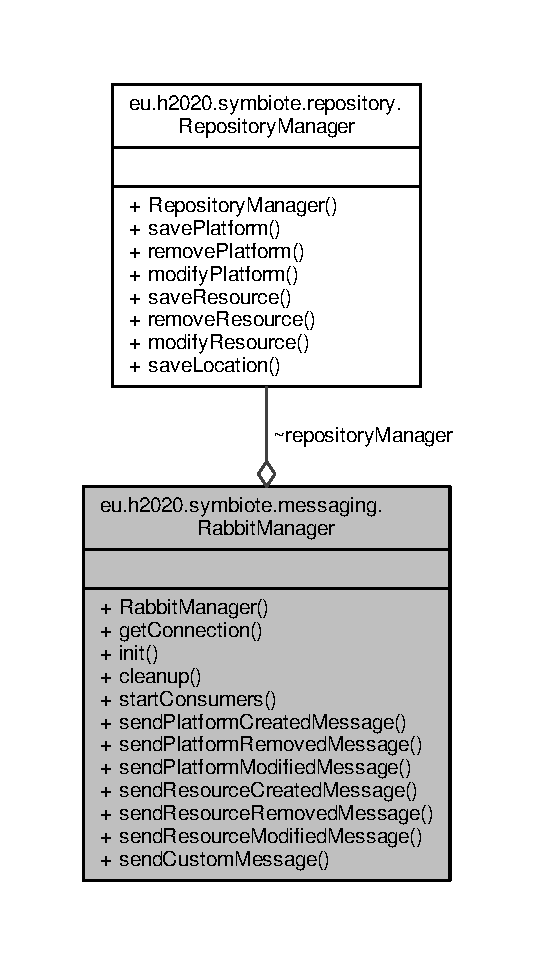
\includegraphics[width=258pt]{classeu_1_1h2020_1_1symbiote_1_1messaging_1_1RabbitManager__coll__graph}
\end{center}
\end{figure}
\subsection*{Public Member Functions}
\begin{DoxyCompactItemize}
\item 
{\bfseries Rabbit\+Manager} (\hyperlink{classeu_1_1h2020_1_1symbiote_1_1repository_1_1RepositoryManager}{Repository\+Manager} repository\+Manager)\hypertarget{classeu_1_1h2020_1_1symbiote_1_1messaging_1_1RabbitManager_ad05170cea6626e742a9b3ff5a359b192}{}\label{classeu_1_1h2020_1_1symbiote_1_1messaging_1_1RabbitManager_ad05170cea6626e742a9b3ff5a359b192}

\item 
Connection \hyperlink{classeu_1_1h2020_1_1symbiote_1_1messaging_1_1RabbitManager_ac6037e07ab7703c98c8a880a1ea5f5cd}{get\+Connection} ()  throws I\+O\+Exception, Timeout\+Exception 
\item 
void \hyperlink{classeu_1_1h2020_1_1symbiote_1_1messaging_1_1RabbitManager_ae6688b10d5858345271d21eda576036c}{init} ()
\item 
void \hyperlink{classeu_1_1h2020_1_1symbiote_1_1messaging_1_1RabbitManager_abf294e221b0bbfc0faa81d38fcec50cd}{cleanup} ()
\item 
void \hyperlink{classeu_1_1h2020_1_1symbiote_1_1messaging_1_1RabbitManager_ab6555364fdd7e95b41802ae24da7f30f}{start\+Consumers} ()
\item 
void {\bfseries send\+Platform\+Created\+Message} (\hyperlink{classeu_1_1h2020_1_1symbiote_1_1model_1_1Platform}{Platform} platform)\hypertarget{classeu_1_1h2020_1_1symbiote_1_1messaging_1_1RabbitManager_ad0733a08e8a207dac36c8ae6a86dfe7e}{}\label{classeu_1_1h2020_1_1symbiote_1_1messaging_1_1RabbitManager_ad0733a08e8a207dac36c8ae6a86dfe7e}

\item 
void {\bfseries send\+Platform\+Removed\+Message} (\hyperlink{classeu_1_1h2020_1_1symbiote_1_1model_1_1Platform}{Platform} platform)\hypertarget{classeu_1_1h2020_1_1symbiote_1_1messaging_1_1RabbitManager_af0a5271ea2607bc84b77f81d70e6dcd7}{}\label{classeu_1_1h2020_1_1symbiote_1_1messaging_1_1RabbitManager_af0a5271ea2607bc84b77f81d70e6dcd7}

\item 
void {\bfseries send\+Platform\+Modified\+Message} (\hyperlink{classeu_1_1h2020_1_1symbiote_1_1model_1_1Platform}{Platform} platform)\hypertarget{classeu_1_1h2020_1_1symbiote_1_1messaging_1_1RabbitManager_ac241cd7e1ec4b33aa0a907b86eecb354}{}\label{classeu_1_1h2020_1_1symbiote_1_1messaging_1_1RabbitManager_ac241cd7e1ec4b33aa0a907b86eecb354}

\item 
void {\bfseries send\+Resource\+Created\+Message} (\hyperlink{classeu_1_1h2020_1_1symbiote_1_1model_1_1Resource}{Resource} resource)\hypertarget{classeu_1_1h2020_1_1symbiote_1_1messaging_1_1RabbitManager_a1499d1a2def21a1c2a405b1448918da7}{}\label{classeu_1_1h2020_1_1symbiote_1_1messaging_1_1RabbitManager_a1499d1a2def21a1c2a405b1448918da7}

\item 
void {\bfseries send\+Resource\+Removed\+Message} (\hyperlink{classeu_1_1h2020_1_1symbiote_1_1model_1_1Resource}{Resource} resource)\hypertarget{classeu_1_1h2020_1_1symbiote_1_1messaging_1_1RabbitManager_aa77dd12749ba669407cdd928eb7138b6}{}\label{classeu_1_1h2020_1_1symbiote_1_1messaging_1_1RabbitManager_aa77dd12749ba669407cdd928eb7138b6}

\item 
void {\bfseries send\+Resource\+Modified\+Message} (\hyperlink{classeu_1_1h2020_1_1symbiote_1_1model_1_1Resource}{Resource} resource)\hypertarget{classeu_1_1h2020_1_1symbiote_1_1messaging_1_1RabbitManager_a05e443fe0be56a424239727cfed231da}{}\label{classeu_1_1h2020_1_1symbiote_1_1messaging_1_1RabbitManager_a05e443fe0be56a424239727cfed231da}

\item 
void {\bfseries send\+Custom\+Message} (String exchange, String routing\+Key, String object\+In\+Json)\hypertarget{classeu_1_1h2020_1_1symbiote_1_1messaging_1_1RabbitManager_a39ec3510289f5e647eb4dab95f82e127}{}\label{classeu_1_1h2020_1_1symbiote_1_1messaging_1_1RabbitManager_a39ec3510289f5e647eb4dab95f82e127}

\end{DoxyCompactItemize}


\subsection{Detailed Description}
Bean used to manage internal communication using Rabbit\+MQ. It is responsible for declaring exchanges and using routing keys from centralized config server. 

Created by mateuszl 

\subsection{Member Function Documentation}
\index{eu\+::h2020\+::symbiote\+::messaging\+::\+Rabbit\+Manager@{eu\+::h2020\+::symbiote\+::messaging\+::\+Rabbit\+Manager}!cleanup@{cleanup}}
\index{cleanup@{cleanup}!eu\+::h2020\+::symbiote\+::messaging\+::\+Rabbit\+Manager@{eu\+::h2020\+::symbiote\+::messaging\+::\+Rabbit\+Manager}}
\subsubsection[{\texorpdfstring{cleanup()}{cleanup()}}]{\setlength{\rightskip}{0pt plus 5cm}void eu.\+h2020.\+symbiote.\+messaging.\+Rabbit\+Manager.\+cleanup (
\begin{DoxyParamCaption}
{}
\end{DoxyParamCaption}
)}\hypertarget{classeu_1_1h2020_1_1symbiote_1_1messaging_1_1RabbitManager_abf294e221b0bbfc0faa81d38fcec50cd}{}\label{classeu_1_1h2020_1_1symbiote_1_1messaging_1_1RabbitManager_abf294e221b0bbfc0faa81d38fcec50cd}
Cleanup method for rabbit -\/ set on pre destroy \index{eu\+::h2020\+::symbiote\+::messaging\+::\+Rabbit\+Manager@{eu\+::h2020\+::symbiote\+::messaging\+::\+Rabbit\+Manager}!get\+Connection@{get\+Connection}}
\index{get\+Connection@{get\+Connection}!eu\+::h2020\+::symbiote\+::messaging\+::\+Rabbit\+Manager@{eu\+::h2020\+::symbiote\+::messaging\+::\+Rabbit\+Manager}}
\subsubsection[{\texorpdfstring{get\+Connection()}{getConnection()}}]{\setlength{\rightskip}{0pt plus 5cm}Connection eu.\+h2020.\+symbiote.\+messaging.\+Rabbit\+Manager.\+get\+Connection (
\begin{DoxyParamCaption}
{}
\end{DoxyParamCaption}
) throws I\+O\+Exception, Timeout\+Exception}\hypertarget{classeu_1_1h2020_1_1symbiote_1_1messaging_1_1RabbitManager_ac6037e07ab7703c98c8a880a1ea5f5cd}{}\label{classeu_1_1h2020_1_1symbiote_1_1messaging_1_1RabbitManager_ac6037e07ab7703c98c8a880a1ea5f5cd}
Initiates connection with Rabbit server using parameters from Config\+Properties


\begin{DoxyExceptions}{Exceptions}
{\em I\+O\+Exception} & \\
\hline
{\em Timeout\+Exception} & \\
\hline
\end{DoxyExceptions}
\index{eu\+::h2020\+::symbiote\+::messaging\+::\+Rabbit\+Manager@{eu\+::h2020\+::symbiote\+::messaging\+::\+Rabbit\+Manager}!init@{init}}
\index{init@{init}!eu\+::h2020\+::symbiote\+::messaging\+::\+Rabbit\+Manager@{eu\+::h2020\+::symbiote\+::messaging\+::\+Rabbit\+Manager}}
\subsubsection[{\texorpdfstring{init()}{init()}}]{\setlength{\rightskip}{0pt plus 5cm}void eu.\+h2020.\+symbiote.\+messaging.\+Rabbit\+Manager.\+init (
\begin{DoxyParamCaption}
{}
\end{DoxyParamCaption}
)}\hypertarget{classeu_1_1h2020_1_1symbiote_1_1messaging_1_1RabbitManager_ae6688b10d5858345271d21eda576036c}{}\label{classeu_1_1h2020_1_1symbiote_1_1messaging_1_1RabbitManager_ae6688b10d5858345271d21eda576036c}
Method creates channel and declares Rabbit exchanges for Platform and Resources. It triggers start of all consumers used in Registry communication. \index{eu\+::h2020\+::symbiote\+::messaging\+::\+Rabbit\+Manager@{eu\+::h2020\+::symbiote\+::messaging\+::\+Rabbit\+Manager}!start\+Consumers@{start\+Consumers}}
\index{start\+Consumers@{start\+Consumers}!eu\+::h2020\+::symbiote\+::messaging\+::\+Rabbit\+Manager@{eu\+::h2020\+::symbiote\+::messaging\+::\+Rabbit\+Manager}}
\subsubsection[{\texorpdfstring{start\+Consumers()}{startConsumers()}}]{\setlength{\rightskip}{0pt plus 5cm}void eu.\+h2020.\+symbiote.\+messaging.\+Rabbit\+Manager.\+start\+Consumers (
\begin{DoxyParamCaption}
{}
\end{DoxyParamCaption}
)}\hypertarget{classeu_1_1h2020_1_1symbiote_1_1messaging_1_1RabbitManager_ab6555364fdd7e95b41802ae24da7f30f}{}\label{classeu_1_1h2020_1_1symbiote_1_1messaging_1_1RabbitManager_ab6555364fdd7e95b41802ae24da7f30f}
Method gathers all of the rabbit consumer starter methods 

The documentation for this class was generated from the following file\+:\begin{DoxyCompactItemize}
\item 
src/main/java/eu/h2020/symbiote/messaging/Rabbit\+Manager.\+java\end{DoxyCompactItemize}

\hypertarget{classeu_1_1h2020_1_1symbiote_1_1RegistryApplication}{}\section{eu.\+h2020.\+symbiote.\+Registry\+Application Class Reference}
\label{classeu_1_1h2020_1_1symbiote_1_1RegistryApplication}\index{eu.\+h2020.\+symbiote.\+Registry\+Application@{eu.\+h2020.\+symbiote.\+Registry\+Application}}


Collaboration diagram for eu.\+h2020.\+symbiote.\+Registry\+Application\+:
\nopagebreak
\begin{figure}[H]
\begin{center}
\leavevmode
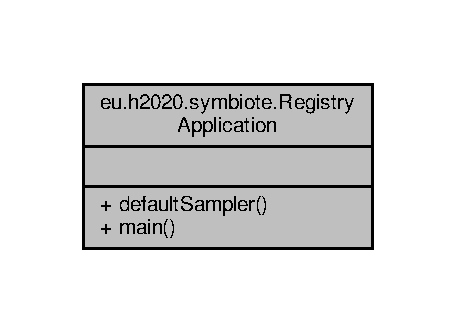
\includegraphics[width=219pt]{classeu_1_1h2020_1_1symbiote_1_1RegistryApplication__coll__graph}
\end{center}
\end{figure}
\subsection*{Classes}
\begin{DoxyCompactItemize}
\item 
class {\bfseries C\+LR}
\end{DoxyCompactItemize}
\subsection*{Public Member Functions}
\begin{DoxyCompactItemize}
\item 
Always\+Sampler {\bfseries default\+Sampler} ()\hypertarget{classeu_1_1h2020_1_1symbiote_1_1RegistryApplication_afd4955b603a321eda1a9b8138093839b}{}\label{classeu_1_1h2020_1_1symbiote_1_1RegistryApplication_afd4955b603a321eda1a9b8138093839b}

\end{DoxyCompactItemize}
\subsection*{Static Public Member Functions}
\begin{DoxyCompactItemize}
\item 
static void {\bfseries main} (String\mbox{[}$\,$\mbox{]} args)\hypertarget{classeu_1_1h2020_1_1symbiote_1_1RegistryApplication_a5ffab7a5e414dd85a6da531224e1501c}{}\label{classeu_1_1h2020_1_1symbiote_1_1RegistryApplication_a5ffab7a5e414dd85a6da531224e1501c}

\end{DoxyCompactItemize}


\subsection{Detailed Description}
Created by mateuszl on 22.\+09.\+2016. 

The documentation for this class was generated from the following file\+:\begin{DoxyCompactItemize}
\item 
src/main/java/eu/h2020/symbiote/Registry\+Application.\+java\end{DoxyCompactItemize}

\hypertarget{classeu_1_1h2020_1_1symbiote_1_1utils_1_1RegistryUtils}{}\section{eu.\+h2020.\+symbiote.\+utils.\+Registry\+Utils Class Reference}
\label{classeu_1_1h2020_1_1symbiote_1_1utils_1_1RegistryUtils}\index{eu.\+h2020.\+symbiote.\+utils.\+Registry\+Utils@{eu.\+h2020.\+symbiote.\+utils.\+Registry\+Utils}}


Collaboration diagram for eu.\+h2020.\+symbiote.\+utils.\+Registry\+Utils\+:
% FIG 0
\subsection*{Static Public Member Functions}
\begin{DoxyCompactItemize}
\item 
static boolean \hyperlink{classeu_1_1h2020_1_1symbiote_1_1utils_1_1RegistryUtils_aa582cda28eb88a92888e378b25323b0a}{validate} (\hyperlink{classeu_1_1h2020_1_1symbiote_1_1model_1_1Platform}{Platform} platform)
\item 
static boolean \hyperlink{classeu_1_1h2020_1_1symbiote_1_1utils_1_1RegistryUtils_a751c1e9ab2152395d5a11c93960ffbf2}{validate} (\hyperlink{classeu_1_1h2020_1_1symbiote_1_1model_1_1Resource}{Resource} resource)
\end{DoxyCompactItemize}


\subsection{Detailed Description}
Utils for manipulating P\+O\+J\+Os in Registry project.

Created by mateuszl on 14.\+02.\+2017. 

\subsection{Member Function Documentation}
\index{eu\+::h2020\+::symbiote\+::utils\+::\+Registry\+Utils@{eu\+::h2020\+::symbiote\+::utils\+::\+Registry\+Utils}!validate@{validate}}
\index{validate@{validate}!eu\+::h2020\+::symbiote\+::utils\+::\+Registry\+Utils@{eu\+::h2020\+::symbiote\+::utils\+::\+Registry\+Utils}}
\subsubsection[{\texorpdfstring{validate(\+Platform platform)}{validate(Platform platform)}}]{\setlength{\rightskip}{0pt plus 5cm}static boolean eu.\+h2020.\+symbiote.\+utils.\+Registry\+Utils.\+validate (
\begin{DoxyParamCaption}
\item[{{\bf Platform}}]{platform}
\end{DoxyParamCaption}
)\hspace{0.3cm}{\ttfamily [static]}}\hypertarget{classeu_1_1h2020_1_1symbiote_1_1utils_1_1RegistryUtils_aa582cda28eb88a92888e378b25323b0a}{}\label{classeu_1_1h2020_1_1symbiote_1_1utils_1_1RegistryUtils_aa582cda28eb88a92888e378b25323b0a}
Checks if given platform has all of the needed fields and that neither is empty.


\begin{DoxyParams}{Parameters}
{\em platform} & platform to check \\
\hline
\end{DoxyParams}
\begin{DoxyReturn}{Returns}
true if it has all the fields and neither is empty 
\end{DoxyReturn}
\index{eu\+::h2020\+::symbiote\+::utils\+::\+Registry\+Utils@{eu\+::h2020\+::symbiote\+::utils\+::\+Registry\+Utils}!validate@{validate}}
\index{validate@{validate}!eu\+::h2020\+::symbiote\+::utils\+::\+Registry\+Utils@{eu\+::h2020\+::symbiote\+::utils\+::\+Registry\+Utils}}
\subsubsection[{\texorpdfstring{validate(\+Resource resource)}{validate(Resource resource)}}]{\setlength{\rightskip}{0pt plus 5cm}static boolean eu.\+h2020.\+symbiote.\+utils.\+Registry\+Utils.\+validate (
\begin{DoxyParamCaption}
\item[{{\bf Resource}}]{resource}
\end{DoxyParamCaption}
)\hspace{0.3cm}{\ttfamily [static]}}\hypertarget{classeu_1_1h2020_1_1symbiote_1_1utils_1_1RegistryUtils_a751c1e9ab2152395d5a11c93960ffbf2}{}\label{classeu_1_1h2020_1_1symbiote_1_1utils_1_1RegistryUtils_a751c1e9ab2152395d5a11c93960ffbf2}
Checks if given resource has all of the needed fields and that neither is empty.


\begin{DoxyParams}{Parameters}
{\em resource} & resource to check \\
\hline
\end{DoxyParams}
\begin{DoxyReturn}{Returns}
true if it has all the fields and neither is empty. 
\end{DoxyReturn}


The documentation for this class was generated from the following file\+:\begin{DoxyCompactItemize}
\item 
src/main/java/eu/h2020/symbiote/utils/Registry\+Utils.\+java\end{DoxyCompactItemize}

\hypertarget{classeu_1_1h2020_1_1symbiote_1_1repository_1_1RepositoryManager}{}\section{eu.\+h2020.\+symbiote.\+repository.\+Repository\+Manager Class Reference}
\label{classeu_1_1h2020_1_1symbiote_1_1repository_1_1RepositoryManager}\index{eu.\+h2020.\+symbiote.\+repository.\+Repository\+Manager@{eu.\+h2020.\+symbiote.\+repository.\+Repository\+Manager}}


Collaboration diagram for eu.\+h2020.\+symbiote.\+repository.\+Repository\+Manager\+:
\nopagebreak
\begin{figure}[H]
\begin{center}
\leavevmode
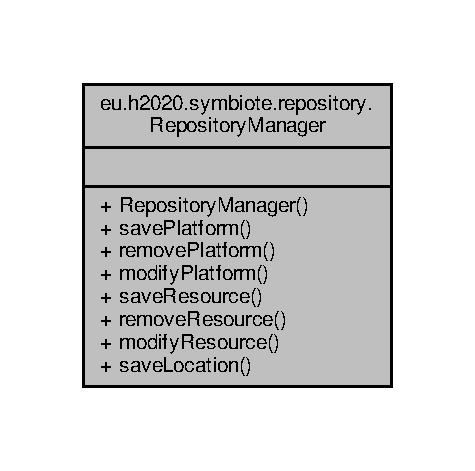
\includegraphics[width=228pt]{classeu_1_1h2020_1_1symbiote_1_1repository_1_1RepositoryManager__coll__graph}
\end{center}
\end{figure}
\subsection*{Public Member Functions}
\begin{DoxyCompactItemize}
\item 
{\bfseries Repository\+Manager} (\hyperlink{interfaceeu_1_1h2020_1_1symbiote_1_1repository_1_1PlatformRepository}{Platform\+Repository} platform\+Repository, \hyperlink{interfaceeu_1_1h2020_1_1symbiote_1_1repository_1_1ResourceRepository}{Resource\+Repository} resource\+Repository, \hyperlink{interfaceeu_1_1h2020_1_1symbiote_1_1repository_1_1LocationRepository}{Location\+Repository} location\+Repository)\hypertarget{classeu_1_1h2020_1_1symbiote_1_1repository_1_1RepositoryManager_a7402e1dfdea6c3e6a0d8b84d4e56b7a6}{}\label{classeu_1_1h2020_1_1symbiote_1_1repository_1_1RepositoryManager_a7402e1dfdea6c3e6a0d8b84d4e56b7a6}

\item 
\hyperlink{classeu_1_1h2020_1_1symbiote_1_1model_1_1PlatformResponse}{Platform\+Response} \hyperlink{classeu_1_1h2020_1_1symbiote_1_1repository_1_1RepositoryManager_a4b0ab3911577e2b2577390e9c0566564}{save\+Platform} (\hyperlink{classeu_1_1h2020_1_1symbiote_1_1model_1_1Platform}{Platform} platform)
\item 
\hyperlink{classeu_1_1h2020_1_1symbiote_1_1model_1_1PlatformResponse}{Platform\+Response} \hyperlink{classeu_1_1h2020_1_1symbiote_1_1repository_1_1RepositoryManager_a3040700dcc9c91da9770fc2c5a96cdd1}{remove\+Platform} (\hyperlink{classeu_1_1h2020_1_1symbiote_1_1model_1_1Platform}{Platform} platform)
\item 
\hyperlink{classeu_1_1h2020_1_1symbiote_1_1model_1_1PlatformResponse}{Platform\+Response} \hyperlink{classeu_1_1h2020_1_1symbiote_1_1repository_1_1RepositoryManager_aeb1e54e87272c6a36188a75ee984d6f4}{modify\+Platform} (\hyperlink{classeu_1_1h2020_1_1symbiote_1_1model_1_1Platform}{Platform} platform)
\item 
\hyperlink{classeu_1_1h2020_1_1symbiote_1_1model_1_1ResourceResponse}{Resource\+Response} \hyperlink{classeu_1_1h2020_1_1symbiote_1_1repository_1_1RepositoryManager_a28f5700428aaffef548549bbccc6672b}{save\+Resource} (\hyperlink{classeu_1_1h2020_1_1symbiote_1_1model_1_1Resource}{Resource} resource)
\item 
\hyperlink{classeu_1_1h2020_1_1symbiote_1_1model_1_1ResourceResponse}{Resource\+Response} \hyperlink{classeu_1_1h2020_1_1symbiote_1_1repository_1_1RepositoryManager_ae2b1a848ec4bc02164d652a910550cc6}{remove\+Resource} (\hyperlink{classeu_1_1h2020_1_1symbiote_1_1model_1_1Resource}{Resource} resource)
\item 
\hyperlink{classeu_1_1h2020_1_1symbiote_1_1model_1_1ResourceResponse}{Resource\+Response} \hyperlink{classeu_1_1h2020_1_1symbiote_1_1repository_1_1RepositoryManager_aa501f5c6448048328ab71d7a9316f4a7}{modify\+Resource} (\hyperlink{classeu_1_1h2020_1_1symbiote_1_1model_1_1Resource}{Resource} resource)
\item 
\hyperlink{classeu_1_1h2020_1_1symbiote_1_1model_1_1Location}{Location} \hyperlink{classeu_1_1h2020_1_1symbiote_1_1repository_1_1RepositoryManager_ab019d153486c163e20cdaa7eaa39c4c0}{save\+Location} (\hyperlink{classeu_1_1h2020_1_1symbiote_1_1model_1_1Location}{Location} location)
\end{DoxyCompactItemize}


\subsection{Detailed Description}
Class managing persistence actions for Platforms, Resources and Locations using Mongo\+DB repositories.

Created by mateuszl 

\subsection{Member Function Documentation}
\index{eu\+::h2020\+::symbiote\+::repository\+::\+Repository\+Manager@{eu\+::h2020\+::symbiote\+::repository\+::\+Repository\+Manager}!modify\+Platform@{modify\+Platform}}
\index{modify\+Platform@{modify\+Platform}!eu\+::h2020\+::symbiote\+::repository\+::\+Repository\+Manager@{eu\+::h2020\+::symbiote\+::repository\+::\+Repository\+Manager}}
\subsubsection[{\texorpdfstring{modify\+Platform(\+Platform platform)}{modifyPlatform(Platform platform)}}]{\setlength{\rightskip}{0pt plus 5cm}{\bf Platform\+Response} eu.\+h2020.\+symbiote.\+repository.\+Repository\+Manager.\+modify\+Platform (
\begin{DoxyParamCaption}
\item[{{\bf Platform}}]{platform}
\end{DoxyParamCaption}
)}\hypertarget{classeu_1_1h2020_1_1symbiote_1_1repository_1_1RepositoryManager_aeb1e54e87272c6a36188a75ee984d6f4}{}\label{classeu_1_1h2020_1_1symbiote_1_1repository_1_1RepositoryManager_aeb1e54e87272c6a36188a75ee984d6f4}
Modifies (existing in mongodb) Platform accordingly to fields in given Platform. It triggers delete and save actions in Platform Repository and if it ends successfully, it returns http status \textquotesingle{}200\textquotesingle{} and new modified Platform object. Url of given platform is appended with \char`\"{}/\char`\"{} if it does not end with it. If given platform has any null field, it is retrieved from DB and fulfilled. If given platform has no ID or has an empty \textquotesingle{}id\textquotesingle{} field the method will return \textquotesingle{}bad request\textquotesingle{} status. If there is no Platform in database with ID same as given one, it returns \textquotesingle{}bad request\textquotesingle{} status. If saving in DB goes wrong it returns \textquotesingle{}internal server error\textquotesingle{} status.


\begin{DoxyParams}{Parameters}
{\em platform} & Platform to remove -\/ in J\+S\+ON format \\
\hline
\end{DoxyParams}
\begin{DoxyReturn}{Returns}
Platform\+Response with Http status code and modified Platform object -\/ in J\+S\+ON format 
\end{DoxyReturn}
\index{eu\+::h2020\+::symbiote\+::repository\+::\+Repository\+Manager@{eu\+::h2020\+::symbiote\+::repository\+::\+Repository\+Manager}!modify\+Resource@{modify\+Resource}}
\index{modify\+Resource@{modify\+Resource}!eu\+::h2020\+::symbiote\+::repository\+::\+Repository\+Manager@{eu\+::h2020\+::symbiote\+::repository\+::\+Repository\+Manager}}
\subsubsection[{\texorpdfstring{modify\+Resource(\+Resource resource)}{modifyResource(Resource resource)}}]{\setlength{\rightskip}{0pt plus 5cm}{\bf Resource\+Response} eu.\+h2020.\+symbiote.\+repository.\+Repository\+Manager.\+modify\+Resource (
\begin{DoxyParamCaption}
\item[{{\bf Resource}}]{resource}
\end{DoxyParamCaption}
)}\hypertarget{classeu_1_1h2020_1_1symbiote_1_1repository_1_1RepositoryManager_aa501f5c6448048328ab71d7a9316f4a7}{}\label{classeu_1_1h2020_1_1symbiote_1_1repository_1_1RepositoryManager_aa501f5c6448048328ab71d7a9316f4a7}
Modifies given resource in Mongo\+DB


\begin{DoxyParams}{Parameters}
{\em resource} & Resource with given properties in J\+S\+ON format \\
\hline
\end{DoxyParams}
\begin{DoxyReturn}{Returns}
Resource\+Response containing Http status code and Modified Resource, in J\+S\+ON format 
\end{DoxyReturn}
\index{eu\+::h2020\+::symbiote\+::repository\+::\+Repository\+Manager@{eu\+::h2020\+::symbiote\+::repository\+::\+Repository\+Manager}!remove\+Platform@{remove\+Platform}}
\index{remove\+Platform@{remove\+Platform}!eu\+::h2020\+::symbiote\+::repository\+::\+Repository\+Manager@{eu\+::h2020\+::symbiote\+::repository\+::\+Repository\+Manager}}
\subsubsection[{\texorpdfstring{remove\+Platform(\+Platform platform)}{removePlatform(Platform platform)}}]{\setlength{\rightskip}{0pt plus 5cm}{\bf Platform\+Response} eu.\+h2020.\+symbiote.\+repository.\+Repository\+Manager.\+remove\+Platform (
\begin{DoxyParamCaption}
\item[{{\bf Platform}}]{platform}
\end{DoxyParamCaption}
)}\hypertarget{classeu_1_1h2020_1_1symbiote_1_1repository_1_1RepositoryManager_a3040700dcc9c91da9770fc2c5a96cdd1}{}\label{classeu_1_1h2020_1_1symbiote_1_1repository_1_1RepositoryManager_a3040700dcc9c91da9770fc2c5a96cdd1}
Removes given Platform from Mongo\+DB. It triggers delete action in Platform Repository and if it ends successfully it returns http status \textquotesingle{}200\textquotesingle{} and removed Platform object. If given platform is null or it has no id or has an empty \textquotesingle{}id\textquotesingle{} field the method will return \textquotesingle{}bad request\textquotesingle{} status. If saving in DB goes wrong it returns \textquotesingle{}internal server error\textquotesingle{} status.


\begin{DoxyParams}{Parameters}
{\em platform} & Platform to remove -\/ in J\+S\+ON format \\
\hline
\end{DoxyParams}
\begin{DoxyReturn}{Returns}
Platform\+Response with Http status code and removed Platform object -\/ in J\+S\+ON format 
\end{DoxyReturn}
\index{eu\+::h2020\+::symbiote\+::repository\+::\+Repository\+Manager@{eu\+::h2020\+::symbiote\+::repository\+::\+Repository\+Manager}!remove\+Resource@{remove\+Resource}}
\index{remove\+Resource@{remove\+Resource}!eu\+::h2020\+::symbiote\+::repository\+::\+Repository\+Manager@{eu\+::h2020\+::symbiote\+::repository\+::\+Repository\+Manager}}
\subsubsection[{\texorpdfstring{remove\+Resource(\+Resource resource)}{removeResource(Resource resource)}}]{\setlength{\rightskip}{0pt plus 5cm}{\bf Resource\+Response} eu.\+h2020.\+symbiote.\+repository.\+Repository\+Manager.\+remove\+Resource (
\begin{DoxyParamCaption}
\item[{{\bf Resource}}]{resource}
\end{DoxyParamCaption}
)}\hypertarget{classeu_1_1h2020_1_1symbiote_1_1repository_1_1RepositoryManager_ae2b1a848ec4bc02164d652a910550cc6}{}\label{classeu_1_1h2020_1_1symbiote_1_1repository_1_1RepositoryManager_ae2b1a848ec4bc02164d652a910550cc6}
Deletes resource from Mongo\+DB


\begin{DoxyParams}{Parameters}
{\em resource} & Resource with given properties in J\+S\+ON format \\
\hline
\end{DoxyParams}
\begin{DoxyReturn}{Returns}
Resource\+Response containing Http status code and Deleted Resource, in J\+S\+ON format 
\end{DoxyReturn}
\index{eu\+::h2020\+::symbiote\+::repository\+::\+Repository\+Manager@{eu\+::h2020\+::symbiote\+::repository\+::\+Repository\+Manager}!save\+Location@{save\+Location}}
\index{save\+Location@{save\+Location}!eu\+::h2020\+::symbiote\+::repository\+::\+Repository\+Manager@{eu\+::h2020\+::symbiote\+::repository\+::\+Repository\+Manager}}
\subsubsection[{\texorpdfstring{save\+Location(\+Location location)}{saveLocation(Location location)}}]{\setlength{\rightskip}{0pt plus 5cm}{\bf Location} eu.\+h2020.\+symbiote.\+repository.\+Repository\+Manager.\+save\+Location (
\begin{DoxyParamCaption}
\item[{{\bf Location}}]{location}
\end{DoxyParamCaption}
)}\hypertarget{classeu_1_1h2020_1_1symbiote_1_1repository_1_1RepositoryManager_ab019d153486c163e20cdaa7eaa39c4c0}{}\label{classeu_1_1h2020_1_1symbiote_1_1repository_1_1RepositoryManager_ab019d153486c163e20cdaa7eaa39c4c0}
Saves in Mongo\+DB given Location.


\begin{DoxyParams}{Parameters}
{\em location} & Location object to save. \\
\hline
\end{DoxyParams}
\begin{DoxyReturn}{Returns}
saved Location with ID field fulfilled. 
\end{DoxyReturn}
\index{eu\+::h2020\+::symbiote\+::repository\+::\+Repository\+Manager@{eu\+::h2020\+::symbiote\+::repository\+::\+Repository\+Manager}!save\+Platform@{save\+Platform}}
\index{save\+Platform@{save\+Platform}!eu\+::h2020\+::symbiote\+::repository\+::\+Repository\+Manager@{eu\+::h2020\+::symbiote\+::repository\+::\+Repository\+Manager}}
\subsubsection[{\texorpdfstring{save\+Platform(\+Platform platform)}{savePlatform(Platform platform)}}]{\setlength{\rightskip}{0pt plus 5cm}{\bf Platform\+Response} eu.\+h2020.\+symbiote.\+repository.\+Repository\+Manager.\+save\+Platform (
\begin{DoxyParamCaption}
\item[{{\bf Platform}}]{platform}
\end{DoxyParamCaption}
)}\hypertarget{classeu_1_1h2020_1_1symbiote_1_1repository_1_1RepositoryManager_a4b0ab3911577e2b2577390e9c0566564}{}\label{classeu_1_1h2020_1_1symbiote_1_1repository_1_1RepositoryManager_a4b0ab3911577e2b2577390e9c0566564}
Saves given Platform in Mongo\+DB. It triggers save action in Platform Repository and if it ends successfully it returns http status \textquotesingle{}200\textquotesingle{} and Platform object with generated ID field. If given platform U\+RL noe ends with \char`\"{}/\char`\"{}, method appends it. If given platform is null or it already has an id the method will return \textquotesingle{}bad request\textquotesingle{} status. If saving in DB goes wrong it returns \textquotesingle{}internal server error\textquotesingle{} status. Url of given platform is appended with \char`\"{}/\char`\"{} if it does not end with it.


\begin{DoxyParams}{Parameters}
{\em platform} & Platform to save -\/ in J\+S\+ON format \\
\hline
\end{DoxyParams}
\begin{DoxyReturn}{Returns}
Platform\+Response with Http status code and Platform object with unique \char`\"{}id\char`\"{} (generated in Mongo\+DB) 
\end{DoxyReturn}
\index{eu\+::h2020\+::symbiote\+::repository\+::\+Repository\+Manager@{eu\+::h2020\+::symbiote\+::repository\+::\+Repository\+Manager}!save\+Resource@{save\+Resource}}
\index{save\+Resource@{save\+Resource}!eu\+::h2020\+::symbiote\+::repository\+::\+Repository\+Manager@{eu\+::h2020\+::symbiote\+::repository\+::\+Repository\+Manager}}
\subsubsection[{\texorpdfstring{save\+Resource(\+Resource resource)}{saveResource(Resource resource)}}]{\setlength{\rightskip}{0pt plus 5cm}{\bf Resource\+Response} eu.\+h2020.\+symbiote.\+repository.\+Repository\+Manager.\+save\+Resource (
\begin{DoxyParamCaption}
\item[{{\bf Resource}}]{resource}
\end{DoxyParamCaption}
)}\hypertarget{classeu_1_1h2020_1_1symbiote_1_1repository_1_1RepositoryManager_a28f5700428aaffef548549bbccc6672b}{}\label{classeu_1_1h2020_1_1symbiote_1_1repository_1_1RepositoryManager_a28f5700428aaffef548549bbccc6672b}
Saves resource in Mongo\+DB. Checks if U\+RL in given resource ends with \char`\"{}/\char`\"{} and if not, appends it. If in database there is no Platform with given Platform\+Id field, the method will return \textquotesingle{}bad request\textquotesingle{} status. If given resource has not null Id field, the method will return \textquotesingle{}bad request\textquotesingle{} status. If in database there is no Platform with given U\+RL same as in given Resource, the method will return \textquotesingle{}bad request\textquotesingle{}. If saving in DB goes wrong it returns \textquotesingle{}internal server error\textquotesingle{} status.


\begin{DoxyParams}{Parameters}
{\em resource} & Resource with given properties in J\+S\+ON format \\
\hline
\end{DoxyParams}
\begin{DoxyReturn}{Returns}
Resource\+Response containing Http status code and Resource with added \textquotesingle{}Id\textquotesingle{} (generated in Mongo\+DB), in J\+S\+ON format 
\end{DoxyReturn}


The documentation for this class was generated from the following file\+:\begin{DoxyCompactItemize}
\item 
src/main/java/eu/h2020/symbiote/repository/Repository\+Manager.\+java\end{DoxyCompactItemize}

\hypertarget{classeu_1_1h2020_1_1symbiote_1_1model_1_1Resource}{}\section{eu.\+h2020.\+symbiote.\+model.\+Resource Class Reference}
\label{classeu_1_1h2020_1_1symbiote_1_1model_1_1Resource}\index{eu.\+h2020.\+symbiote.\+model.\+Resource@{eu.\+h2020.\+symbiote.\+model.\+Resource}}


Collaboration diagram for eu.\+h2020.\+symbiote.\+model.\+Resource\+:
% FIG 0
\subsection*{Public Member Functions}
\begin{DoxyCompactItemize}
\item 
String \hyperlink{classeu_1_1h2020_1_1symbiote_1_1model_1_1Resource_a6d2b00f0e94b55cce1daff002012369c}{get\+Id} ()
\item 
void \hyperlink{classeu_1_1h2020_1_1symbiote_1_1model_1_1Resource_a209815ba7cdb6b82334e664eb4c38708}{set\+Id} (String id)
\item 
String \hyperlink{classeu_1_1h2020_1_1symbiote_1_1model_1_1Resource_a7332986d4dfa4ca233f705659f166f2c}{get\+Name} ()
\item 
void \hyperlink{classeu_1_1h2020_1_1symbiote_1_1model_1_1Resource_ad2cd06bcbfa928adead9017509cc2e78}{set\+Name} (String name)
\item 
String \hyperlink{classeu_1_1h2020_1_1symbiote_1_1model_1_1Resource_a0bd495e4c9a10fac6e885de268b5ad76}{get\+Owner} ()
\item 
void \hyperlink{classeu_1_1h2020_1_1symbiote_1_1model_1_1Resource_a4391365a9ef765fb9c96e8243a45fafb}{set\+Owner} (String owner)
\item 
String \hyperlink{classeu_1_1h2020_1_1symbiote_1_1model_1_1Resource_ae2ce583e094c18bca236027602739049}{get\+Description} ()
\item 
void \hyperlink{classeu_1_1h2020_1_1symbiote_1_1model_1_1Resource_a19349909b51f43be943fcc3ebc078009}{set\+Description} (String description)
\item 
List$<$ String $>$ \hyperlink{classeu_1_1h2020_1_1symbiote_1_1model_1_1Resource_a2aaf59e1be5b0c974a31e106adfa6c43}{get\+Observed\+Properties} ()
\item 
void \hyperlink{classeu_1_1h2020_1_1symbiote_1_1model_1_1Resource_a826dbee60cf539ffbf1a088496ac7e11}{set\+Observed\+Properties} (List$<$ String $>$ observed\+Properties)
\item 
String \hyperlink{classeu_1_1h2020_1_1symbiote_1_1model_1_1Resource_a4a0c05d9007f2216c55ddc32a44f467b}{get\+Resource\+U\+RL} ()
\item 
void \hyperlink{classeu_1_1h2020_1_1symbiote_1_1model_1_1Resource_a27d7401a8087bf902fd575039d574d0c}{set\+Resource\+U\+RL} (String resource\+U\+RL)
\item 
\hyperlink{classeu_1_1h2020_1_1symbiote_1_1model_1_1Location}{Location} \hyperlink{classeu_1_1h2020_1_1symbiote_1_1model_1_1Resource_acfb7ead093f1ed692640c99daba8fc6c}{get\+Location} ()
\item 
void \hyperlink{classeu_1_1h2020_1_1symbiote_1_1model_1_1Resource_a14eba3bd0171783f32d6d4446768905d}{set\+Location} (\hyperlink{classeu_1_1h2020_1_1symbiote_1_1model_1_1Location}{Location} location)
\item 
String \hyperlink{classeu_1_1h2020_1_1symbiote_1_1model_1_1Resource_a1e5912a2e60f0d2dcda674f26ebe871b}{get\+Feature\+Of\+Interest} ()
\item 
void \hyperlink{classeu_1_1h2020_1_1symbiote_1_1model_1_1Resource_abcfd5b3b2e1515ca7e9eb50eeb7ed0cf}{set\+Feature\+Of\+Interest} (String feature\+Of\+Interest)
\item 
String \hyperlink{classeu_1_1h2020_1_1symbiote_1_1model_1_1Resource_a97e847fb787ea9fe1d16d8bd702deece}{get\+Platform\+Id} ()
\item 
void \hyperlink{classeu_1_1h2020_1_1symbiote_1_1model_1_1Resource_a4f3c37b066d6e6587912fa1f1240048f}{set\+Platform\+Id} (String platform\+Id)
\end{DoxyCompactItemize}


\subsection{Detailed Description}
Registry \hyperlink{classeu_1_1h2020_1_1symbiote_1_1model_1_1Resource}{Resource} object

Created by mateuszl 

\subsection{Member Function Documentation}
\index{eu\+::h2020\+::symbiote\+::model\+::\+Resource@{eu\+::h2020\+::symbiote\+::model\+::\+Resource}!get\+Description@{get\+Description}}
\index{get\+Description@{get\+Description}!eu\+::h2020\+::symbiote\+::model\+::\+Resource@{eu\+::h2020\+::symbiote\+::model\+::\+Resource}}
\subsubsection[{\texorpdfstring{get\+Description()}{getDescription()}}]{\setlength{\rightskip}{0pt plus 5cm}String eu.\+h2020.\+symbiote.\+model.\+Resource.\+get\+Description (
\begin{DoxyParamCaption}
{}
\end{DoxyParamCaption}
)}\hypertarget{classeu_1_1h2020_1_1symbiote_1_1model_1_1Resource_ae2ce583e094c18bca236027602739049}{}\label{classeu_1_1h2020_1_1symbiote_1_1model_1_1Resource_ae2ce583e094c18bca236027602739049}
\begin{DoxyReturn}{Returns}

\end{DoxyReturn}
\index{eu\+::h2020\+::symbiote\+::model\+::\+Resource@{eu\+::h2020\+::symbiote\+::model\+::\+Resource}!get\+Feature\+Of\+Interest@{get\+Feature\+Of\+Interest}}
\index{get\+Feature\+Of\+Interest@{get\+Feature\+Of\+Interest}!eu\+::h2020\+::symbiote\+::model\+::\+Resource@{eu\+::h2020\+::symbiote\+::model\+::\+Resource}}
\subsubsection[{\texorpdfstring{get\+Feature\+Of\+Interest()}{getFeatureOfInterest()}}]{\setlength{\rightskip}{0pt plus 5cm}String eu.\+h2020.\+symbiote.\+model.\+Resource.\+get\+Feature\+Of\+Interest (
\begin{DoxyParamCaption}
{}
\end{DoxyParamCaption}
)}\hypertarget{classeu_1_1h2020_1_1symbiote_1_1model_1_1Resource_a1e5912a2e60f0d2dcda674f26ebe871b}{}\label{classeu_1_1h2020_1_1symbiote_1_1model_1_1Resource_a1e5912a2e60f0d2dcda674f26ebe871b}
\begin{DoxyReturn}{Returns}

\end{DoxyReturn}
\index{eu\+::h2020\+::symbiote\+::model\+::\+Resource@{eu\+::h2020\+::symbiote\+::model\+::\+Resource}!get\+Id@{get\+Id}}
\index{get\+Id@{get\+Id}!eu\+::h2020\+::symbiote\+::model\+::\+Resource@{eu\+::h2020\+::symbiote\+::model\+::\+Resource}}
\subsubsection[{\texorpdfstring{get\+Id()}{getId()}}]{\setlength{\rightskip}{0pt plus 5cm}String eu.\+h2020.\+symbiote.\+model.\+Resource.\+get\+Id (
\begin{DoxyParamCaption}
{}
\end{DoxyParamCaption}
)}\hypertarget{classeu_1_1h2020_1_1symbiote_1_1model_1_1Resource_a6d2b00f0e94b55cce1daff002012369c}{}\label{classeu_1_1h2020_1_1symbiote_1_1model_1_1Resource_a6d2b00f0e94b55cce1daff002012369c}
\begin{DoxyReturn}{Returns}

\end{DoxyReturn}
\index{eu\+::h2020\+::symbiote\+::model\+::\+Resource@{eu\+::h2020\+::symbiote\+::model\+::\+Resource}!get\+Location@{get\+Location}}
\index{get\+Location@{get\+Location}!eu\+::h2020\+::symbiote\+::model\+::\+Resource@{eu\+::h2020\+::symbiote\+::model\+::\+Resource}}
\subsubsection[{\texorpdfstring{get\+Location()}{getLocation()}}]{\setlength{\rightskip}{0pt plus 5cm}{\bf Location} eu.\+h2020.\+symbiote.\+model.\+Resource.\+get\+Location (
\begin{DoxyParamCaption}
{}
\end{DoxyParamCaption}
)}\hypertarget{classeu_1_1h2020_1_1symbiote_1_1model_1_1Resource_acfb7ead093f1ed692640c99daba8fc6c}{}\label{classeu_1_1h2020_1_1symbiote_1_1model_1_1Resource_acfb7ead093f1ed692640c99daba8fc6c}
\begin{DoxyReturn}{Returns}

\end{DoxyReturn}
\index{eu\+::h2020\+::symbiote\+::model\+::\+Resource@{eu\+::h2020\+::symbiote\+::model\+::\+Resource}!get\+Name@{get\+Name}}
\index{get\+Name@{get\+Name}!eu\+::h2020\+::symbiote\+::model\+::\+Resource@{eu\+::h2020\+::symbiote\+::model\+::\+Resource}}
\subsubsection[{\texorpdfstring{get\+Name()}{getName()}}]{\setlength{\rightskip}{0pt plus 5cm}String eu.\+h2020.\+symbiote.\+model.\+Resource.\+get\+Name (
\begin{DoxyParamCaption}
{}
\end{DoxyParamCaption}
)}\hypertarget{classeu_1_1h2020_1_1symbiote_1_1model_1_1Resource_a7332986d4dfa4ca233f705659f166f2c}{}\label{classeu_1_1h2020_1_1symbiote_1_1model_1_1Resource_a7332986d4dfa4ca233f705659f166f2c}
\begin{DoxyReturn}{Returns}

\end{DoxyReturn}
\index{eu\+::h2020\+::symbiote\+::model\+::\+Resource@{eu\+::h2020\+::symbiote\+::model\+::\+Resource}!get\+Observed\+Properties@{get\+Observed\+Properties}}
\index{get\+Observed\+Properties@{get\+Observed\+Properties}!eu\+::h2020\+::symbiote\+::model\+::\+Resource@{eu\+::h2020\+::symbiote\+::model\+::\+Resource}}
\subsubsection[{\texorpdfstring{get\+Observed\+Properties()}{getObservedProperties()}}]{\setlength{\rightskip}{0pt plus 5cm}List$<$String$>$ eu.\+h2020.\+symbiote.\+model.\+Resource.\+get\+Observed\+Properties (
\begin{DoxyParamCaption}
{}
\end{DoxyParamCaption}
)}\hypertarget{classeu_1_1h2020_1_1symbiote_1_1model_1_1Resource_a2aaf59e1be5b0c974a31e106adfa6c43}{}\label{classeu_1_1h2020_1_1symbiote_1_1model_1_1Resource_a2aaf59e1be5b0c974a31e106adfa6c43}
\begin{DoxyReturn}{Returns}

\end{DoxyReturn}
\index{eu\+::h2020\+::symbiote\+::model\+::\+Resource@{eu\+::h2020\+::symbiote\+::model\+::\+Resource}!get\+Owner@{get\+Owner}}
\index{get\+Owner@{get\+Owner}!eu\+::h2020\+::symbiote\+::model\+::\+Resource@{eu\+::h2020\+::symbiote\+::model\+::\+Resource}}
\subsubsection[{\texorpdfstring{get\+Owner()}{getOwner()}}]{\setlength{\rightskip}{0pt plus 5cm}String eu.\+h2020.\+symbiote.\+model.\+Resource.\+get\+Owner (
\begin{DoxyParamCaption}
{}
\end{DoxyParamCaption}
)}\hypertarget{classeu_1_1h2020_1_1symbiote_1_1model_1_1Resource_a0bd495e4c9a10fac6e885de268b5ad76}{}\label{classeu_1_1h2020_1_1symbiote_1_1model_1_1Resource_a0bd495e4c9a10fac6e885de268b5ad76}
\begin{DoxyReturn}{Returns}

\end{DoxyReturn}
\index{eu\+::h2020\+::symbiote\+::model\+::\+Resource@{eu\+::h2020\+::symbiote\+::model\+::\+Resource}!get\+Platform\+Id@{get\+Platform\+Id}}
\index{get\+Platform\+Id@{get\+Platform\+Id}!eu\+::h2020\+::symbiote\+::model\+::\+Resource@{eu\+::h2020\+::symbiote\+::model\+::\+Resource}}
\subsubsection[{\texorpdfstring{get\+Platform\+Id()}{getPlatformId()}}]{\setlength{\rightskip}{0pt plus 5cm}String eu.\+h2020.\+symbiote.\+model.\+Resource.\+get\+Platform\+Id (
\begin{DoxyParamCaption}
{}
\end{DoxyParamCaption}
)}\hypertarget{classeu_1_1h2020_1_1symbiote_1_1model_1_1Resource_a97e847fb787ea9fe1d16d8bd702deece}{}\label{classeu_1_1h2020_1_1symbiote_1_1model_1_1Resource_a97e847fb787ea9fe1d16d8bd702deece}
\begin{DoxyReturn}{Returns}

\end{DoxyReturn}
\index{eu\+::h2020\+::symbiote\+::model\+::\+Resource@{eu\+::h2020\+::symbiote\+::model\+::\+Resource}!get\+Resource\+U\+RL@{get\+Resource\+U\+RL}}
\index{get\+Resource\+U\+RL@{get\+Resource\+U\+RL}!eu\+::h2020\+::symbiote\+::model\+::\+Resource@{eu\+::h2020\+::symbiote\+::model\+::\+Resource}}
\subsubsection[{\texorpdfstring{get\+Resource\+U\+R\+L()}{getResourceURL()}}]{\setlength{\rightskip}{0pt plus 5cm}String eu.\+h2020.\+symbiote.\+model.\+Resource.\+get\+Resource\+U\+RL (
\begin{DoxyParamCaption}
{}
\end{DoxyParamCaption}
)}\hypertarget{classeu_1_1h2020_1_1symbiote_1_1model_1_1Resource_a4a0c05d9007f2216c55ddc32a44f467b}{}\label{classeu_1_1h2020_1_1symbiote_1_1model_1_1Resource_a4a0c05d9007f2216c55ddc32a44f467b}
\begin{DoxyReturn}{Returns}

\end{DoxyReturn}
\index{eu\+::h2020\+::symbiote\+::model\+::\+Resource@{eu\+::h2020\+::symbiote\+::model\+::\+Resource}!set\+Description@{set\+Description}}
\index{set\+Description@{set\+Description}!eu\+::h2020\+::symbiote\+::model\+::\+Resource@{eu\+::h2020\+::symbiote\+::model\+::\+Resource}}
\subsubsection[{\texorpdfstring{set\+Description(\+String description)}{setDescription(String description)}}]{\setlength{\rightskip}{0pt plus 5cm}void eu.\+h2020.\+symbiote.\+model.\+Resource.\+set\+Description (
\begin{DoxyParamCaption}
\item[{String}]{description}
\end{DoxyParamCaption}
)}\hypertarget{classeu_1_1h2020_1_1symbiote_1_1model_1_1Resource_a19349909b51f43be943fcc3ebc078009}{}\label{classeu_1_1h2020_1_1symbiote_1_1model_1_1Resource_a19349909b51f43be943fcc3ebc078009}

\begin{DoxyParams}{Parameters}
{\em description} & \\
\hline
\end{DoxyParams}
\index{eu\+::h2020\+::symbiote\+::model\+::\+Resource@{eu\+::h2020\+::symbiote\+::model\+::\+Resource}!set\+Feature\+Of\+Interest@{set\+Feature\+Of\+Interest}}
\index{set\+Feature\+Of\+Interest@{set\+Feature\+Of\+Interest}!eu\+::h2020\+::symbiote\+::model\+::\+Resource@{eu\+::h2020\+::symbiote\+::model\+::\+Resource}}
\subsubsection[{\texorpdfstring{set\+Feature\+Of\+Interest(\+String feature\+Of\+Interest)}{setFeatureOfInterest(String featureOfInterest)}}]{\setlength{\rightskip}{0pt plus 5cm}void eu.\+h2020.\+symbiote.\+model.\+Resource.\+set\+Feature\+Of\+Interest (
\begin{DoxyParamCaption}
\item[{String}]{feature\+Of\+Interest}
\end{DoxyParamCaption}
)}\hypertarget{classeu_1_1h2020_1_1symbiote_1_1model_1_1Resource_abcfd5b3b2e1515ca7e9eb50eeb7ed0cf}{}\label{classeu_1_1h2020_1_1symbiote_1_1model_1_1Resource_abcfd5b3b2e1515ca7e9eb50eeb7ed0cf}

\begin{DoxyParams}{Parameters}
{\em feature\+Of\+Interest} & \\
\hline
\end{DoxyParams}
\index{eu\+::h2020\+::symbiote\+::model\+::\+Resource@{eu\+::h2020\+::symbiote\+::model\+::\+Resource}!set\+Id@{set\+Id}}
\index{set\+Id@{set\+Id}!eu\+::h2020\+::symbiote\+::model\+::\+Resource@{eu\+::h2020\+::symbiote\+::model\+::\+Resource}}
\subsubsection[{\texorpdfstring{set\+Id(\+String id)}{setId(String id)}}]{\setlength{\rightskip}{0pt plus 5cm}void eu.\+h2020.\+symbiote.\+model.\+Resource.\+set\+Id (
\begin{DoxyParamCaption}
\item[{String}]{id}
\end{DoxyParamCaption}
)}\hypertarget{classeu_1_1h2020_1_1symbiote_1_1model_1_1Resource_a209815ba7cdb6b82334e664eb4c38708}{}\label{classeu_1_1h2020_1_1symbiote_1_1model_1_1Resource_a209815ba7cdb6b82334e664eb4c38708}

\begin{DoxyParams}{Parameters}
{\em id} & \\
\hline
\end{DoxyParams}
\index{eu\+::h2020\+::symbiote\+::model\+::\+Resource@{eu\+::h2020\+::symbiote\+::model\+::\+Resource}!set\+Location@{set\+Location}}
\index{set\+Location@{set\+Location}!eu\+::h2020\+::symbiote\+::model\+::\+Resource@{eu\+::h2020\+::symbiote\+::model\+::\+Resource}}
\subsubsection[{\texorpdfstring{set\+Location(\+Location location)}{setLocation(Location location)}}]{\setlength{\rightskip}{0pt plus 5cm}void eu.\+h2020.\+symbiote.\+model.\+Resource.\+set\+Location (
\begin{DoxyParamCaption}
\item[{{\bf Location}}]{location}
\end{DoxyParamCaption}
)}\hypertarget{classeu_1_1h2020_1_1symbiote_1_1model_1_1Resource_a14eba3bd0171783f32d6d4446768905d}{}\label{classeu_1_1h2020_1_1symbiote_1_1model_1_1Resource_a14eba3bd0171783f32d6d4446768905d}

\begin{DoxyParams}{Parameters}
{\em location} & \\
\hline
\end{DoxyParams}
\index{eu\+::h2020\+::symbiote\+::model\+::\+Resource@{eu\+::h2020\+::symbiote\+::model\+::\+Resource}!set\+Name@{set\+Name}}
\index{set\+Name@{set\+Name}!eu\+::h2020\+::symbiote\+::model\+::\+Resource@{eu\+::h2020\+::symbiote\+::model\+::\+Resource}}
\subsubsection[{\texorpdfstring{set\+Name(\+String name)}{setName(String name)}}]{\setlength{\rightskip}{0pt plus 5cm}void eu.\+h2020.\+symbiote.\+model.\+Resource.\+set\+Name (
\begin{DoxyParamCaption}
\item[{String}]{name}
\end{DoxyParamCaption}
)}\hypertarget{classeu_1_1h2020_1_1symbiote_1_1model_1_1Resource_ad2cd06bcbfa928adead9017509cc2e78}{}\label{classeu_1_1h2020_1_1symbiote_1_1model_1_1Resource_ad2cd06bcbfa928adead9017509cc2e78}

\begin{DoxyParams}{Parameters}
{\em name} & \\
\hline
\end{DoxyParams}
\index{eu\+::h2020\+::symbiote\+::model\+::\+Resource@{eu\+::h2020\+::symbiote\+::model\+::\+Resource}!set\+Observed\+Properties@{set\+Observed\+Properties}}
\index{set\+Observed\+Properties@{set\+Observed\+Properties}!eu\+::h2020\+::symbiote\+::model\+::\+Resource@{eu\+::h2020\+::symbiote\+::model\+::\+Resource}}
\subsubsection[{\texorpdfstring{set\+Observed\+Properties(\+List$<$ String $>$ observed\+Properties)}{setObservedProperties(List< String > observedProperties)}}]{\setlength{\rightskip}{0pt plus 5cm}void eu.\+h2020.\+symbiote.\+model.\+Resource.\+set\+Observed\+Properties (
\begin{DoxyParamCaption}
\item[{List$<$ String $>$}]{observed\+Properties}
\end{DoxyParamCaption}
)}\hypertarget{classeu_1_1h2020_1_1symbiote_1_1model_1_1Resource_a826dbee60cf539ffbf1a088496ac7e11}{}\label{classeu_1_1h2020_1_1symbiote_1_1model_1_1Resource_a826dbee60cf539ffbf1a088496ac7e11}

\begin{DoxyParams}{Parameters}
{\em observed\+Properties} & \\
\hline
\end{DoxyParams}
\index{eu\+::h2020\+::symbiote\+::model\+::\+Resource@{eu\+::h2020\+::symbiote\+::model\+::\+Resource}!set\+Owner@{set\+Owner}}
\index{set\+Owner@{set\+Owner}!eu\+::h2020\+::symbiote\+::model\+::\+Resource@{eu\+::h2020\+::symbiote\+::model\+::\+Resource}}
\subsubsection[{\texorpdfstring{set\+Owner(\+String owner)}{setOwner(String owner)}}]{\setlength{\rightskip}{0pt plus 5cm}void eu.\+h2020.\+symbiote.\+model.\+Resource.\+set\+Owner (
\begin{DoxyParamCaption}
\item[{String}]{owner}
\end{DoxyParamCaption}
)}\hypertarget{classeu_1_1h2020_1_1symbiote_1_1model_1_1Resource_a4391365a9ef765fb9c96e8243a45fafb}{}\label{classeu_1_1h2020_1_1symbiote_1_1model_1_1Resource_a4391365a9ef765fb9c96e8243a45fafb}

\begin{DoxyParams}{Parameters}
{\em owner} & \\
\hline
\end{DoxyParams}
\index{eu\+::h2020\+::symbiote\+::model\+::\+Resource@{eu\+::h2020\+::symbiote\+::model\+::\+Resource}!set\+Platform\+Id@{set\+Platform\+Id}}
\index{set\+Platform\+Id@{set\+Platform\+Id}!eu\+::h2020\+::symbiote\+::model\+::\+Resource@{eu\+::h2020\+::symbiote\+::model\+::\+Resource}}
\subsubsection[{\texorpdfstring{set\+Platform\+Id(\+String platform\+Id)}{setPlatformId(String platformId)}}]{\setlength{\rightskip}{0pt plus 5cm}void eu.\+h2020.\+symbiote.\+model.\+Resource.\+set\+Platform\+Id (
\begin{DoxyParamCaption}
\item[{String}]{platform\+Id}
\end{DoxyParamCaption}
)}\hypertarget{classeu_1_1h2020_1_1symbiote_1_1model_1_1Resource_a4f3c37b066d6e6587912fa1f1240048f}{}\label{classeu_1_1h2020_1_1symbiote_1_1model_1_1Resource_a4f3c37b066d6e6587912fa1f1240048f}

\begin{DoxyParams}{Parameters}
{\em platform\+Id} & \\
\hline
\end{DoxyParams}
\index{eu\+::h2020\+::symbiote\+::model\+::\+Resource@{eu\+::h2020\+::symbiote\+::model\+::\+Resource}!set\+Resource\+U\+RL@{set\+Resource\+U\+RL}}
\index{set\+Resource\+U\+RL@{set\+Resource\+U\+RL}!eu\+::h2020\+::symbiote\+::model\+::\+Resource@{eu\+::h2020\+::symbiote\+::model\+::\+Resource}}
\subsubsection[{\texorpdfstring{set\+Resource\+U\+R\+L(\+String resource\+U\+R\+L)}{setResourceURL(String resourceURL)}}]{\setlength{\rightskip}{0pt plus 5cm}void eu.\+h2020.\+symbiote.\+model.\+Resource.\+set\+Resource\+U\+RL (
\begin{DoxyParamCaption}
\item[{String}]{resource\+U\+RL}
\end{DoxyParamCaption}
)}\hypertarget{classeu_1_1h2020_1_1symbiote_1_1model_1_1Resource_a27d7401a8087bf902fd575039d574d0c}{}\label{classeu_1_1h2020_1_1symbiote_1_1model_1_1Resource_a27d7401a8087bf902fd575039d574d0c}

\begin{DoxyParams}{Parameters}
{\em resource\+U\+RL} & \\
\hline
\end{DoxyParams}


The documentation for this class was generated from the following file\+:\begin{DoxyCompactItemize}
\item 
src/main/java/eu/h2020/symbiote/model/Resource.\+java\end{DoxyCompactItemize}

\hypertarget{classeu_1_1h2020_1_1symbiote_1_1messaging_1_1ResourceCreationRequestConsumer}{}\section{eu.\+h2020.\+symbiote.\+messaging.\+Resource\+Creation\+Request\+Consumer Class Reference}
\label{classeu_1_1h2020_1_1symbiote_1_1messaging_1_1ResourceCreationRequestConsumer}\index{eu.\+h2020.\+symbiote.\+messaging.\+Resource\+Creation\+Request\+Consumer@{eu.\+h2020.\+symbiote.\+messaging.\+Resource\+Creation\+Request\+Consumer}}


Inheritance diagram for eu.\+h2020.\+symbiote.\+messaging.\+Resource\+Creation\+Request\+Consumer\+:
\nopagebreak
\begin{figure}[H]
\begin{center}
\leavevmode
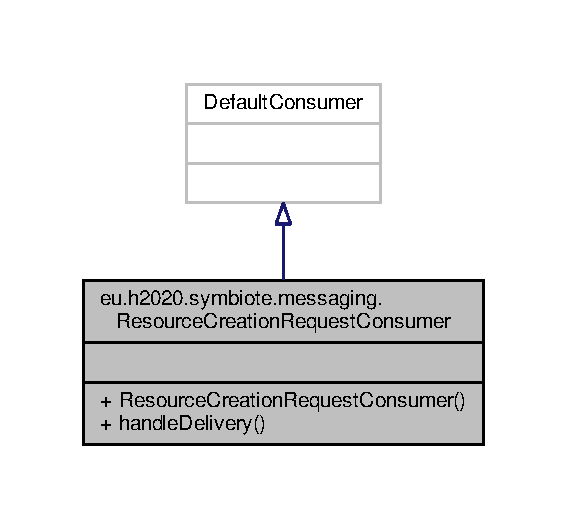
\includegraphics[width=272pt]{classeu_1_1h2020_1_1symbiote_1_1messaging_1_1ResourceCreationRequestConsumer__inherit__graph}
\end{center}
\end{figure}


Collaboration diagram for eu.\+h2020.\+symbiote.\+messaging.\+Resource\+Creation\+Request\+Consumer\+:
\nopagebreak
\begin{figure}[H]
\begin{center}
\leavevmode
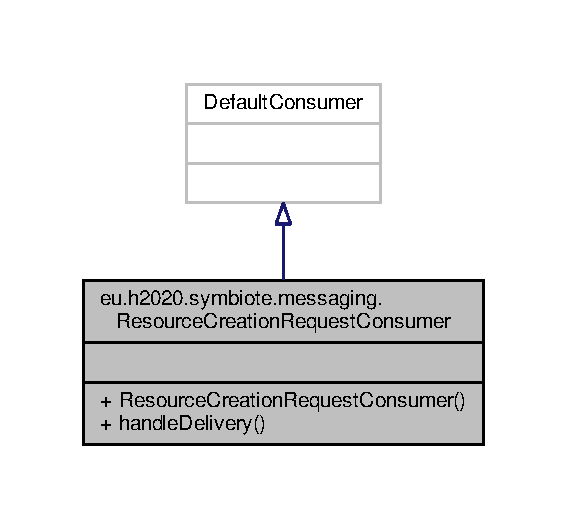
\includegraphics[width=272pt]{classeu_1_1h2020_1_1symbiote_1_1messaging_1_1ResourceCreationRequestConsumer__coll__graph}
\end{center}
\end{figure}
\subsection*{Public Member Functions}
\begin{DoxyCompactItemize}
\item 
\hyperlink{classeu_1_1h2020_1_1symbiote_1_1messaging_1_1ResourceCreationRequestConsumer_ad02c4274f1fa39b858e7c68120704e94}{Resource\+Creation\+Request\+Consumer} (Channel channel, \hyperlink{classeu_1_1h2020_1_1symbiote_1_1repository_1_1RepositoryManager}{Repository\+Manager} repository\+Manager, \hyperlink{classeu_1_1h2020_1_1symbiote_1_1messaging_1_1RabbitManager}{Rabbit\+Manager} rabbit\+Manager)
\item 
void \hyperlink{classeu_1_1h2020_1_1symbiote_1_1messaging_1_1ResourceCreationRequestConsumer_ac2192f2c6e6d644dc1ba1ca91a2fbb3c}{handle\+Delivery} (String consumer\+Tag, Envelope envelope, A\+M\+Q\+P.\+Basic\+Properties properties, byte\mbox{[}$\,$\mbox{]} body)  throws I\+O\+Exception 
\end{DoxyCompactItemize}


\subsection{Detailed Description}
Rabbit\+MQ Consumer implementation used for Resource Creation actions

Created by mateuszl 

\subsection{Constructor \& Destructor Documentation}
\index{eu\+::h2020\+::symbiote\+::messaging\+::\+Resource\+Creation\+Request\+Consumer@{eu\+::h2020\+::symbiote\+::messaging\+::\+Resource\+Creation\+Request\+Consumer}!Resource\+Creation\+Request\+Consumer@{Resource\+Creation\+Request\+Consumer}}
\index{Resource\+Creation\+Request\+Consumer@{Resource\+Creation\+Request\+Consumer}!eu\+::h2020\+::symbiote\+::messaging\+::\+Resource\+Creation\+Request\+Consumer@{eu\+::h2020\+::symbiote\+::messaging\+::\+Resource\+Creation\+Request\+Consumer}}
\subsubsection[{\texorpdfstring{Resource\+Creation\+Request\+Consumer(\+Channel channel, Repository\+Manager repository\+Manager, Rabbit\+Manager rabbit\+Manager)}{ResourceCreationRequestConsumer(Channel channel, RepositoryManager repositoryManager, RabbitManager rabbitManager)}}]{\setlength{\rightskip}{0pt plus 5cm}eu.\+h2020.\+symbiote.\+messaging.\+Resource\+Creation\+Request\+Consumer.\+Resource\+Creation\+Request\+Consumer (
\begin{DoxyParamCaption}
\item[{Channel}]{channel, }
\item[{{\bf Repository\+Manager}}]{repository\+Manager, }
\item[{{\bf Rabbit\+Manager}}]{rabbit\+Manager}
\end{DoxyParamCaption}
)}\hypertarget{classeu_1_1h2020_1_1symbiote_1_1messaging_1_1ResourceCreationRequestConsumer_ad02c4274f1fa39b858e7c68120704e94}{}\label{classeu_1_1h2020_1_1symbiote_1_1messaging_1_1ResourceCreationRequestConsumer_ad02c4274f1fa39b858e7c68120704e94}
Constructs a new instance and records its association to the passed-\/in channel. Managers beans passed as parameters because of lack of possibility to inject it to consumer.


\begin{DoxyParams}{Parameters}
{\em channel} & the channel to which this consumer is attached \\
\hline
{\em rabbit\+Manager} & rabbit manager bean passed for access to messages manager \\
\hline
{\em repository\+Manager} & repository manager bean passed for persistence actions \\
\hline
\end{DoxyParams}


\subsection{Member Function Documentation}
\index{eu\+::h2020\+::symbiote\+::messaging\+::\+Resource\+Creation\+Request\+Consumer@{eu\+::h2020\+::symbiote\+::messaging\+::\+Resource\+Creation\+Request\+Consumer}!handle\+Delivery@{handle\+Delivery}}
\index{handle\+Delivery@{handle\+Delivery}!eu\+::h2020\+::symbiote\+::messaging\+::\+Resource\+Creation\+Request\+Consumer@{eu\+::h2020\+::symbiote\+::messaging\+::\+Resource\+Creation\+Request\+Consumer}}
\subsubsection[{\texorpdfstring{handle\+Delivery(\+String consumer\+Tag, Envelope envelope, A\+M\+Q\+P.\+Basic\+Properties properties, byte[] body)}{handleDelivery(String consumerTag, Envelope envelope, AMQP.BasicProperties properties, byte[] body)}}]{\setlength{\rightskip}{0pt plus 5cm}void eu.\+h2020.\+symbiote.\+messaging.\+Resource\+Creation\+Request\+Consumer.\+handle\+Delivery (
\begin{DoxyParamCaption}
\item[{String}]{consumer\+Tag, }
\item[{Envelope}]{envelope, }
\item[{A\+M\+Q\+P.\+Basic\+Properties}]{properties, }
\item[{byte\mbox{[}$\,$\mbox{]}}]{body}
\end{DoxyParamCaption}
) throws I\+O\+Exception}\hypertarget{classeu_1_1h2020_1_1symbiote_1_1messaging_1_1ResourceCreationRequestConsumer_ac2192f2c6e6d644dc1ba1ca91a2fbb3c}{}\label{classeu_1_1h2020_1_1symbiote_1_1messaging_1_1ResourceCreationRequestConsumer_ac2192f2c6e6d644dc1ba1ca91a2fbb3c}
Called when a {\ttfamily {\bfseries basic.\+deliver}} is received for this consumer.


\begin{DoxyParams}{Parameters}
{\em consumer\+Tag} & the {\itshape consumer tag} associated with the consumer \\
\hline
{\em envelope} & packaging data for the message \\
\hline
{\em properties} & content header data for the message \\
\hline
{\em body} & the message body (opaque, client-\/specific byte array) \\
\hline
\end{DoxyParams}

\begin{DoxyExceptions}{Exceptions}
{\em I\+O\+Exception} & if the consumer encounters an I/O error while processing the message \\
\hline
\end{DoxyExceptions}
\begin{DoxySeeAlso}{See also}
Envelope 
\end{DoxySeeAlso}


The documentation for this class was generated from the following file\+:\begin{DoxyCompactItemize}
\item 
src/main/java/eu/h2020/symbiote/messaging/Resource\+Creation\+Request\+Consumer.\+java\end{DoxyCompactItemize}

\hypertarget{classeu_1_1h2020_1_1symbiote_1_1messaging_1_1ResourceModificationRequestConsumer}{}\section{eu.\+h2020.\+symbiote.\+messaging.\+Resource\+Modification\+Request\+Consumer Class Reference}
\label{classeu_1_1h2020_1_1symbiote_1_1messaging_1_1ResourceModificationRequestConsumer}\index{eu.\+h2020.\+symbiote.\+messaging.\+Resource\+Modification\+Request\+Consumer@{eu.\+h2020.\+symbiote.\+messaging.\+Resource\+Modification\+Request\+Consumer}}


Inheritance diagram for eu.\+h2020.\+symbiote.\+messaging.\+Resource\+Modification\+Request\+Consumer\+:
% FIG 0


Collaboration diagram for eu.\+h2020.\+symbiote.\+messaging.\+Resource\+Modification\+Request\+Consumer\+:
% FIG 1
\subsection*{Public Member Functions}
\begin{DoxyCompactItemize}
\item 
\hyperlink{classeu_1_1h2020_1_1symbiote_1_1messaging_1_1ResourceModificationRequestConsumer_a9edfd7dcca58ed1988bd26d9dd913191}{Resource\+Modification\+Request\+Consumer} (Channel channel, \hyperlink{classeu_1_1h2020_1_1symbiote_1_1repository_1_1RepositoryManager}{Repository\+Manager} repository\+Manager, \hyperlink{classeu_1_1h2020_1_1symbiote_1_1messaging_1_1RabbitManager}{Rabbit\+Manager} rabbit\+Manager)
\item 
void \hyperlink{classeu_1_1h2020_1_1symbiote_1_1messaging_1_1ResourceModificationRequestConsumer_a814265326818232c50a1b91a4b6e347b}{handle\+Delivery} (String consumer\+Tag, Envelope envelope, A\+M\+Q\+P.\+Basic\+Properties properties, byte\mbox{[}$\,$\mbox{]} body)  throws I\+O\+Exception 
\end{DoxyCompactItemize}


\subsection{Detailed Description}
Rabbit\+MQ Consumer implementation used for Resource Modification actions 

\subsection{Constructor \& Destructor Documentation}
\index{eu\+::h2020\+::symbiote\+::messaging\+::\+Resource\+Modification\+Request\+Consumer@{eu\+::h2020\+::symbiote\+::messaging\+::\+Resource\+Modification\+Request\+Consumer}!Resource\+Modification\+Request\+Consumer@{Resource\+Modification\+Request\+Consumer}}
\index{Resource\+Modification\+Request\+Consumer@{Resource\+Modification\+Request\+Consumer}!eu\+::h2020\+::symbiote\+::messaging\+::\+Resource\+Modification\+Request\+Consumer@{eu\+::h2020\+::symbiote\+::messaging\+::\+Resource\+Modification\+Request\+Consumer}}
\subsubsection[{\texorpdfstring{Resource\+Modification\+Request\+Consumer(\+Channel channel, Repository\+Manager repository\+Manager, Rabbit\+Manager rabbit\+Manager)}{ResourceModificationRequestConsumer(Channel channel, RepositoryManager repositoryManager, RabbitManager rabbitManager)}}]{\setlength{\rightskip}{0pt plus 5cm}eu.\+h2020.\+symbiote.\+messaging.\+Resource\+Modification\+Request\+Consumer.\+Resource\+Modification\+Request\+Consumer (
\begin{DoxyParamCaption}
\item[{Channel}]{channel, }
\item[{{\bf Repository\+Manager}}]{repository\+Manager, }
\item[{{\bf Rabbit\+Manager}}]{rabbit\+Manager}
\end{DoxyParamCaption}
)}\hypertarget{classeu_1_1h2020_1_1symbiote_1_1messaging_1_1ResourceModificationRequestConsumer_a9edfd7dcca58ed1988bd26d9dd913191}{}\label{classeu_1_1h2020_1_1symbiote_1_1messaging_1_1ResourceModificationRequestConsumer_a9edfd7dcca58ed1988bd26d9dd913191}
Constructs a new instance and records its association to the passed-\/in channel. Managers beans passed as parameters because of lack of possibility to inject it to consumer.


\begin{DoxyParams}{Parameters}
{\em channel} & the channel to which this consumer is attached \\
\hline
{\em rabbit\+Manager} & rabbit manager bean passed for access to messages manager \\
\hline
{\em repository\+Manager} & repository manager bean passed for persistence actions \\
\hline
\end{DoxyParams}


\subsection{Member Function Documentation}
\index{eu\+::h2020\+::symbiote\+::messaging\+::\+Resource\+Modification\+Request\+Consumer@{eu\+::h2020\+::symbiote\+::messaging\+::\+Resource\+Modification\+Request\+Consumer}!handle\+Delivery@{handle\+Delivery}}
\index{handle\+Delivery@{handle\+Delivery}!eu\+::h2020\+::symbiote\+::messaging\+::\+Resource\+Modification\+Request\+Consumer@{eu\+::h2020\+::symbiote\+::messaging\+::\+Resource\+Modification\+Request\+Consumer}}
\subsubsection[{\texorpdfstring{handle\+Delivery(\+String consumer\+Tag, Envelope envelope, A\+M\+Q\+P.\+Basic\+Properties properties, byte[] body)}{handleDelivery(String consumerTag, Envelope envelope, AMQP.BasicProperties properties, byte[] body)}}]{\setlength{\rightskip}{0pt plus 5cm}void eu.\+h2020.\+symbiote.\+messaging.\+Resource\+Modification\+Request\+Consumer.\+handle\+Delivery (
\begin{DoxyParamCaption}
\item[{String}]{consumer\+Tag, }
\item[{Envelope}]{envelope, }
\item[{A\+M\+Q\+P.\+Basic\+Properties}]{properties, }
\item[{byte\mbox{[}$\,$\mbox{]}}]{body}
\end{DoxyParamCaption}
) throws I\+O\+Exception}\hypertarget{classeu_1_1h2020_1_1symbiote_1_1messaging_1_1ResourceModificationRequestConsumer_a814265326818232c50a1b91a4b6e347b}{}\label{classeu_1_1h2020_1_1symbiote_1_1messaging_1_1ResourceModificationRequestConsumer_a814265326818232c50a1b91a4b6e347b}
Called when a {\ttfamily {\bfseries basic.\+deliver}} is received for this consumer. 
\begin{DoxyParams}{Parameters}
{\em consumer\+Tag} & the {\itshape consumer tag} associated with the consumer \\
\hline
{\em envelope} & packaging data for the message \\
\hline
{\em properties} & content header data for the message \\
\hline
{\em body} & the message body (opaque, client-\/specific byte array) \\
\hline
\end{DoxyParams}

\begin{DoxyExceptions}{Exceptions}
{\em I\+O\+Exception} & if the consumer encounters an I/O error while processing the message \\
\hline
\end{DoxyExceptions}
\begin{DoxySeeAlso}{See also}
Envelope 
\end{DoxySeeAlso}


The documentation for this class was generated from the following file\+:\begin{DoxyCompactItemize}
\item 
src/main/java/eu/h2020/symbiote/messaging/Resource\+Modification\+Request\+Consumer.\+java\end{DoxyCompactItemize}

\hypertarget{classeu_1_1h2020_1_1symbiote_1_1messaging_1_1ResourceRemovalRequestConsumer}{}\section{eu.\+h2020.\+symbiote.\+messaging.\+Resource\+Removal\+Request\+Consumer Class Reference}
\label{classeu_1_1h2020_1_1symbiote_1_1messaging_1_1ResourceRemovalRequestConsumer}\index{eu.\+h2020.\+symbiote.\+messaging.\+Resource\+Removal\+Request\+Consumer@{eu.\+h2020.\+symbiote.\+messaging.\+Resource\+Removal\+Request\+Consumer}}


Inheritance diagram for eu.\+h2020.\+symbiote.\+messaging.\+Resource\+Removal\+Request\+Consumer\+:
% FIG 0


Collaboration diagram for eu.\+h2020.\+symbiote.\+messaging.\+Resource\+Removal\+Request\+Consumer\+:
% FIG 1
\subsection*{Public Member Functions}
\begin{DoxyCompactItemize}
\item 
\hyperlink{classeu_1_1h2020_1_1symbiote_1_1messaging_1_1ResourceRemovalRequestConsumer_aba5553aba270fe213d42a950e5c3ccd6}{Resource\+Removal\+Request\+Consumer} (Channel channel, \hyperlink{classeu_1_1h2020_1_1symbiote_1_1repository_1_1RepositoryManager}{Repository\+Manager} repository\+Manager, \hyperlink{classeu_1_1h2020_1_1symbiote_1_1messaging_1_1RabbitManager}{Rabbit\+Manager} rabbit\+Manager)
\item 
void \hyperlink{classeu_1_1h2020_1_1symbiote_1_1messaging_1_1ResourceRemovalRequestConsumer_acddf45d794a218a11e496d11e47dd01c}{handle\+Delivery} (String consumer\+Tag, Envelope envelope, A\+M\+Q\+P.\+Basic\+Properties properties, byte\mbox{[}$\,$\mbox{]} body)  throws I\+O\+Exception 
\end{DoxyCompactItemize}


\subsection{Detailed Description}
Rabbit\+MQ Consumer implementation used for Resource Removal actions 

\subsection{Constructor \& Destructor Documentation}
\index{eu\+::h2020\+::symbiote\+::messaging\+::\+Resource\+Removal\+Request\+Consumer@{eu\+::h2020\+::symbiote\+::messaging\+::\+Resource\+Removal\+Request\+Consumer}!Resource\+Removal\+Request\+Consumer@{Resource\+Removal\+Request\+Consumer}}
\index{Resource\+Removal\+Request\+Consumer@{Resource\+Removal\+Request\+Consumer}!eu\+::h2020\+::symbiote\+::messaging\+::\+Resource\+Removal\+Request\+Consumer@{eu\+::h2020\+::symbiote\+::messaging\+::\+Resource\+Removal\+Request\+Consumer}}
\subsubsection[{\texorpdfstring{Resource\+Removal\+Request\+Consumer(\+Channel channel, Repository\+Manager repository\+Manager, Rabbit\+Manager rabbit\+Manager)}{ResourceRemovalRequestConsumer(Channel channel, RepositoryManager repositoryManager, RabbitManager rabbitManager)}}]{\setlength{\rightskip}{0pt plus 5cm}eu.\+h2020.\+symbiote.\+messaging.\+Resource\+Removal\+Request\+Consumer.\+Resource\+Removal\+Request\+Consumer (
\begin{DoxyParamCaption}
\item[{Channel}]{channel, }
\item[{{\bf Repository\+Manager}}]{repository\+Manager, }
\item[{{\bf Rabbit\+Manager}}]{rabbit\+Manager}
\end{DoxyParamCaption}
)}\hypertarget{classeu_1_1h2020_1_1symbiote_1_1messaging_1_1ResourceRemovalRequestConsumer_aba5553aba270fe213d42a950e5c3ccd6}{}\label{classeu_1_1h2020_1_1symbiote_1_1messaging_1_1ResourceRemovalRequestConsumer_aba5553aba270fe213d42a950e5c3ccd6}
Constructs a new instance and records its association to the passed-\/in channel. Managers beans passed as parameters because of lack of possibility to inject it to consumer.


\begin{DoxyParams}{Parameters}
{\em channel} & the channel to which this consumer is attached \\
\hline
{\em rabbit\+Manager} & rabbit manager bean passed for access to messages manager \\
\hline
{\em repository\+Manager} & repository manager bean passed for persistence actions \\
\hline
\end{DoxyParams}


\subsection{Member Function Documentation}
\index{eu\+::h2020\+::symbiote\+::messaging\+::\+Resource\+Removal\+Request\+Consumer@{eu\+::h2020\+::symbiote\+::messaging\+::\+Resource\+Removal\+Request\+Consumer}!handle\+Delivery@{handle\+Delivery}}
\index{handle\+Delivery@{handle\+Delivery}!eu\+::h2020\+::symbiote\+::messaging\+::\+Resource\+Removal\+Request\+Consumer@{eu\+::h2020\+::symbiote\+::messaging\+::\+Resource\+Removal\+Request\+Consumer}}
\subsubsection[{\texorpdfstring{handle\+Delivery(\+String consumer\+Tag, Envelope envelope, A\+M\+Q\+P.\+Basic\+Properties properties, byte[] body)}{handleDelivery(String consumerTag, Envelope envelope, AMQP.BasicProperties properties, byte[] body)}}]{\setlength{\rightskip}{0pt plus 5cm}void eu.\+h2020.\+symbiote.\+messaging.\+Resource\+Removal\+Request\+Consumer.\+handle\+Delivery (
\begin{DoxyParamCaption}
\item[{String}]{consumer\+Tag, }
\item[{Envelope}]{envelope, }
\item[{A\+M\+Q\+P.\+Basic\+Properties}]{properties, }
\item[{byte\mbox{[}$\,$\mbox{]}}]{body}
\end{DoxyParamCaption}
) throws I\+O\+Exception}\hypertarget{classeu_1_1h2020_1_1symbiote_1_1messaging_1_1ResourceRemovalRequestConsumer_acddf45d794a218a11e496d11e47dd01c}{}\label{classeu_1_1h2020_1_1symbiote_1_1messaging_1_1ResourceRemovalRequestConsumer_acddf45d794a218a11e496d11e47dd01c}
Called when a {\ttfamily {\bfseries basic.\+deliver}} is received for this consumer. 
\begin{DoxyParams}{Parameters}
{\em consumer\+Tag} & the {\itshape consumer tag} associated with the consumer \\
\hline
{\em envelope} & packaging data for the message \\
\hline
{\em properties} & content header data for the message \\
\hline
{\em body} & the message body (opaque, client-\/specific byte array) \\
\hline
\end{DoxyParams}

\begin{DoxyExceptions}{Exceptions}
{\em I\+O\+Exception} & if the consumer encounters an I/O error while processing the message \\
\hline
\end{DoxyExceptions}
\begin{DoxySeeAlso}{See also}
Envelope 
\end{DoxySeeAlso}


The documentation for this class was generated from the following file\+:\begin{DoxyCompactItemize}
\item 
src/main/java/eu/h2020/symbiote/messaging/Resource\+Removal\+Request\+Consumer.\+java\end{DoxyCompactItemize}

\hypertarget{interfaceeu_1_1h2020_1_1symbiote_1_1repository_1_1ResourceRepository}{}\section{eu.\+h2020.\+symbiote.\+repository.\+Resource\+Repository Interface Reference}
\label{interfaceeu_1_1h2020_1_1symbiote_1_1repository_1_1ResourceRepository}\index{eu.\+h2020.\+symbiote.\+repository.\+Resource\+Repository@{eu.\+h2020.\+symbiote.\+repository.\+Resource\+Repository}}


Inheritance diagram for eu.\+h2020.\+symbiote.\+repository.\+Resource\+Repository\+:
% FIG 0


Collaboration diagram for eu.\+h2020.\+symbiote.\+repository.\+Resource\+Repository\+:
% FIG 1
\subsection*{Public Member Functions}
\begin{DoxyCompactItemize}
\item 
List$<$ \hyperlink{classeu_1_1h2020_1_1symbiote_1_1model_1_1Resource}{Resource} $>$ {\bfseries find\+By\+Platform\+Id} (String platform\+Id)\hypertarget{interfaceeu_1_1h2020_1_1symbiote_1_1repository_1_1ResourceRepository_aec7bce58cf66e21ad20c28041306c089}{}\label{interfaceeu_1_1h2020_1_1symbiote_1_1repository_1_1ResourceRepository_aec7bce58cf66e21ad20c28041306c089}

\end{DoxyCompactItemize}


\subsection{Detailed Description}
Registry Mongo\+DB Persistence layer for Resource objects

Created by mateuszl 

The documentation for this interface was generated from the following file\+:\begin{DoxyCompactItemize}
\item 
src/main/java/eu/h2020/symbiote/repository/Resource\+Repository.\+java\end{DoxyCompactItemize}

\hypertarget{classeu_1_1h2020_1_1symbiote_1_1model_1_1ResourceResponse}{}\section{eu.\+h2020.\+symbiote.\+model.\+Resource\+Response Class Reference}
\label{classeu_1_1h2020_1_1symbiote_1_1model_1_1ResourceResponse}\index{eu.\+h2020.\+symbiote.\+model.\+Resource\+Response@{eu.\+h2020.\+symbiote.\+model.\+Resource\+Response}}


Collaboration diagram for eu.\+h2020.\+symbiote.\+model.\+Resource\+Response\+:
% FIG 0
\subsection*{Public Member Functions}
\begin{DoxyCompactItemize}
\item 
{\bfseries Resource\+Response} (int status, \hyperlink{classeu_1_1h2020_1_1symbiote_1_1model_1_1Resource}{Resource} resource)\hypertarget{classeu_1_1h2020_1_1symbiote_1_1model_1_1ResourceResponse_ad0141ca2e9efa0c7e25e40fcf62a476e}{}\label{classeu_1_1h2020_1_1symbiote_1_1model_1_1ResourceResponse_ad0141ca2e9efa0c7e25e40fcf62a476e}

\item 
int \hyperlink{classeu_1_1h2020_1_1symbiote_1_1model_1_1ResourceResponse_a291fd5f67222ea0f011793defaab2683}{get\+Status} ()
\item 
void \hyperlink{classeu_1_1h2020_1_1symbiote_1_1model_1_1ResourceResponse_ae7de4f16857ef5c7ed1d272684d2aa8d}{set\+Status} (int status)
\item 
\hyperlink{classeu_1_1h2020_1_1symbiote_1_1model_1_1Resource}{Resource} \hyperlink{classeu_1_1h2020_1_1symbiote_1_1model_1_1ResourceResponse_ac366edd9f5b18a37ad1f1935e5cc60f5}{get\+Resource} ()
\item 
void \hyperlink{classeu_1_1h2020_1_1symbiote_1_1model_1_1ResourceResponse_a65d8ae38a592038757a450b0e3bfe52b}{set\+Resource} (\hyperlink{classeu_1_1h2020_1_1symbiote_1_1model_1_1Resource}{Resource} resource)
\end{DoxyCompactItemize}


\subsection{Detailed Description}
Class used as a response to R\+PC call requesting resource actions 

\subsection{Member Function Documentation}
\index{eu\+::h2020\+::symbiote\+::model\+::\+Resource\+Response@{eu\+::h2020\+::symbiote\+::model\+::\+Resource\+Response}!get\+Resource@{get\+Resource}}
\index{get\+Resource@{get\+Resource}!eu\+::h2020\+::symbiote\+::model\+::\+Resource\+Response@{eu\+::h2020\+::symbiote\+::model\+::\+Resource\+Response}}
\subsubsection[{\texorpdfstring{get\+Resource()}{getResource()}}]{\setlength{\rightskip}{0pt plus 5cm}{\bf Resource} eu.\+h2020.\+symbiote.\+model.\+Resource\+Response.\+get\+Resource (
\begin{DoxyParamCaption}
{}
\end{DoxyParamCaption}
)}\hypertarget{classeu_1_1h2020_1_1symbiote_1_1model_1_1ResourceResponse_ac366edd9f5b18a37ad1f1935e5cc60f5}{}\label{classeu_1_1h2020_1_1symbiote_1_1model_1_1ResourceResponse_ac366edd9f5b18a37ad1f1935e5cc60f5}
\begin{DoxyReturn}{Returns}

\end{DoxyReturn}
\index{eu\+::h2020\+::symbiote\+::model\+::\+Resource\+Response@{eu\+::h2020\+::symbiote\+::model\+::\+Resource\+Response}!get\+Status@{get\+Status}}
\index{get\+Status@{get\+Status}!eu\+::h2020\+::symbiote\+::model\+::\+Resource\+Response@{eu\+::h2020\+::symbiote\+::model\+::\+Resource\+Response}}
\subsubsection[{\texorpdfstring{get\+Status()}{getStatus()}}]{\setlength{\rightskip}{0pt plus 5cm}int eu.\+h2020.\+symbiote.\+model.\+Resource\+Response.\+get\+Status (
\begin{DoxyParamCaption}
{}
\end{DoxyParamCaption}
)}\hypertarget{classeu_1_1h2020_1_1symbiote_1_1model_1_1ResourceResponse_a291fd5f67222ea0f011793defaab2683}{}\label{classeu_1_1h2020_1_1symbiote_1_1model_1_1ResourceResponse_a291fd5f67222ea0f011793defaab2683}
\begin{DoxyReturn}{Returns}

\end{DoxyReturn}
\index{eu\+::h2020\+::symbiote\+::model\+::\+Resource\+Response@{eu\+::h2020\+::symbiote\+::model\+::\+Resource\+Response}!set\+Resource@{set\+Resource}}
\index{set\+Resource@{set\+Resource}!eu\+::h2020\+::symbiote\+::model\+::\+Resource\+Response@{eu\+::h2020\+::symbiote\+::model\+::\+Resource\+Response}}
\subsubsection[{\texorpdfstring{set\+Resource(\+Resource resource)}{setResource(Resource resource)}}]{\setlength{\rightskip}{0pt plus 5cm}void eu.\+h2020.\+symbiote.\+model.\+Resource\+Response.\+set\+Resource (
\begin{DoxyParamCaption}
\item[{{\bf Resource}}]{resource}
\end{DoxyParamCaption}
)}\hypertarget{classeu_1_1h2020_1_1symbiote_1_1model_1_1ResourceResponse_a65d8ae38a592038757a450b0e3bfe52b}{}\label{classeu_1_1h2020_1_1symbiote_1_1model_1_1ResourceResponse_a65d8ae38a592038757a450b0e3bfe52b}

\begin{DoxyParams}{Parameters}
{\em resource} & \\
\hline
\end{DoxyParams}
\index{eu\+::h2020\+::symbiote\+::model\+::\+Resource\+Response@{eu\+::h2020\+::symbiote\+::model\+::\+Resource\+Response}!set\+Status@{set\+Status}}
\index{set\+Status@{set\+Status}!eu\+::h2020\+::symbiote\+::model\+::\+Resource\+Response@{eu\+::h2020\+::symbiote\+::model\+::\+Resource\+Response}}
\subsubsection[{\texorpdfstring{set\+Status(int status)}{setStatus(int status)}}]{\setlength{\rightskip}{0pt plus 5cm}void eu.\+h2020.\+symbiote.\+model.\+Resource\+Response.\+set\+Status (
\begin{DoxyParamCaption}
\item[{int}]{status}
\end{DoxyParamCaption}
)}\hypertarget{classeu_1_1h2020_1_1symbiote_1_1model_1_1ResourceResponse_ae7de4f16857ef5c7ed1d272684d2aa8d}{}\label{classeu_1_1h2020_1_1symbiote_1_1model_1_1ResourceResponse_ae7de4f16857ef5c7ed1d272684d2aa8d}

\begin{DoxyParams}{Parameters}
{\em status} & \\
\hline
\end{DoxyParams}


The documentation for this class was generated from the following file\+:\begin{DoxyCompactItemize}
\item 
src/main/java/eu/h2020/symbiote/model/Resource\+Response.\+java\end{DoxyCompactItemize}

%--- End generated contents ---

% Index
\backmatter
\newpage
\phantomsection
\clearemptydoublepage
\addcontentsline{toc}{chapter}{Index}
\printindex

\end{document}
